\documentclass[usenatbib]{mn2e}
\usepackage{float}
\usepackage[pdftex]{graphicx}
\usepackage[utf8]{inputenc}
\usepackage{rotating}
\newcommand{\ol}[1]{ {\overline{#1}}}
\newcommand{\lu}{\,h^{-1}{\rm kpc}}
\renewcommand{\vec}[1]{ {\bmath #1} } 
\newcommand{\e}{{\rm e}}
\newcommand{\dd}{{\rm d}}
\newcommand{\ap}[1]{\textcolor{magenta}{#1}}
\def\gsim{ \lower .75ex \hbox{$\sim$} \llap{\raise .27ex \hbox{$>$}} }
\def\lsim{ \lower .75ex \hbox{$\sim$} \llap{\raise .27ex \hbox{$<$}} }

% Individual page for figures
\usepackage{afterpage}

% Fancy merger rate symbol:
\usepackage{amssymb}
\usepackage{amsmath}
\usepackage[amssymb]{SIunits} 

% Make font much more compact
\usepackage{times}

% Compact lists (compactitem):
\usepackage{paralist}

% References highlighted in blue (include "draft" option for troubleshooting)
\usepackage[bookmarks,bookmarksnumbered,colorlinks=true,citecolor=blue,linkcolor=blue]{hyperref}
\usepackage{color}

% Line break inside table cell
\usepackage{pbox}

% Vertical spaces in table
\usepackage{booktabs}

% Tables with notes, etc.
\usepackage[flushleft]{threeparttable}

% Blocks of comments
\usepackage{comment} 

% Color highlighting
\definecolor{darkgreen}{rgb}{0.0, 0.5, 0.0}
\newcommand{\highlight}[1]{{\color{darkgreen} #1}}

% Custom commands, to be used inside math environment:
\newcommand{\Msun}{{\rm M_{\odot}}}

\setlength{\topmargin}{-1.2cm}

\renewcommand{\thefootnote}{\fnsymbol{footnote}}
\newcommand{\Matrix}[1]{\mathsf{#1}}



\usepackage{booktabs}
\usepackage{hhline}
\usepackage{breqn}
\usepackage{standalone}
\usepackage{dcolumn}
	\newcolumntype{d}[1]{D{.}{.}{#1}}
\usepackage{tabularx}
\usepackage{booktabs}
\usepackage{microtype}
% \usepackage{algpseudocode}
\usepackage[]{algorithm2e}
\usepackage[update,prepend]{epstopdf}
\epstopdfsetup{outdir=./figures/finalized/}
% the search path of the figures for this latex file 
% REMEMBER to add / at the END of the path
\graphicspath{{figures/finalized/}}
% \graphicspath{{./figures/finalized}{figures/drafts/}}

\newcommand{\mc}[1]{\multicolumn{1}{c}{#1}} % handy shortcut macro
%-----------------------------------------------------------------------
\def\Hmat{\mathbf{\it H}}
\def\apjl{ApJL }
\def\aj{AJ }
\def\apj{ApJ }
\def\pasp{PASP }
\def\spie{SPIE }
\def\apjs{ApJS }
\def\araa{ARAA }
\def\aap{A\&A }
\def\nat{Nature }
\def\mnras{MNRAS }
\def\mnrasl{MNRASL }
\providecommand{\eprint}[1]{\href{http://arxiv.org/abs/#1}{#1}}
\providecommand{\adsurl}[1]{\href{#1}{ADS}}
\providecommand{\ISBN}[1]{\href{http://cosmologist.info/ISBN/#1}{ISBN: #1}} 
%-----------------------------------------------------------------------
\title[
	Did we see self-interacting dark matter or statistical noise?]
{Did we see self-interacting dark matter or statistical noise? The galaxy-dark
	matter offsets of the galaxy clusters
	in the Illustris simulation}
\author[Karen Y. Ng et al.]{Karen Y. Ng,$^{1}$
	Annalisa P. Pillepich,$^{2}$ 
	William A. Dawson,$^{3}$ 
	D. Wittman,$^{1}$
	\newauthor Lars Hernquist,$^{2}$
}
\begin{document}
\date{arXiv} \pagerange{\pageref{firstpage}--\pageref{lastpage}}
\pubyear{2015} \maketitle\label{firstpage}
\begin{abstract} 
	Assuming that dark matter has a zero interacting cross section, how likely is
	it for us to see the offset values between dark matter and galaxies 
	from real data? 
	This paper formulates a test using cluster data in the cosmological 
	simulation, the Illustris simulation, to examine that hypothesis. 
	% Galaxy clusters, which mainly compose of dark matter (DM), 
	% can be rare test beds for the particle properties of DM.
	% However, the continuous merger and accretion events of clusters also
	% complicate the modeling of galaxy clusters.
	% With uncertainties coming from various modeling choices and observational 
	% constraints, we need to carefully account for the
	% uncertainties for us to give meaningful quantitative constraints from 
	% the studies of galaxy clusters. In this paper, 
	% we test various summary statistics of the member galaxy components
	% of galaxy clusters by computing them from the data from a cosmological simulation,
	% the Illustris simulation. 
	We examine the uncertainties of the different summary statistics, and see
	if the galaxy population have statistics consistent with those of the DM
	population. TODO: result summary.
	We found that the uncertainty of the offset resulting from projection effects 
	are non-negligible and vary in unpredictable ways. 
\end{abstract}

\begin{keywords}
	galaxy clusters, dark matter, statistics 
\end{keywords}



\section{INTRODUCTION} 
During the latest stage of structure formation, the universe gave birth to
non-linear, hierarchical structures known as galaxy clusters. 
These clusters, made up of dark matter, galaxies and hot gas,
are constantly accreting mass, merging and evolving with their
environments. Bright galaxies that belong to a galaxy cluster or group, in 
particular, highlight the overdensities of the underlying dark matter (DM) 
distribution. 

% Peaks, summary statistics 
% Modeling galaxy clusters - distributions, peaks, centroids 

In these dense regions of the clusters, the rates of particle
interactions can be enhanced, including the long-suspected self-interaction of DM
particles (hereafter, SIDM).  
Many papers have used the offsets between the summary statistics of the DM
density and the galaxy density to give constraints on 
the self-interaction cross
section, i.e. $\sigma_{\rm SIDM}$, of dark matter. 
A lot of observational studies focus on using merging galaxy clusters
as they assume the high collisional velocity should increase the chance
of detecting the effects of SIDM.
By assuming galaxies being relatively collisionless $\sigma_{\rm gal} \approx 0$, 
any offset of the DM population from the galaxy provides $\sigma_{\rm SIDM}$ 
relative to $\sigma_{\rm gal} \approx 0 \centi\meter^2$. 
These observational studies include \cite{Markevitch2004} and \cite{Bradac2006b}  
reporting an offset of 25 kpc for the Bullet Cluster;  
\cite{Dawson2013} reporting an offset of 129 kpc and 47 kpc for the southern
and the northern subcluster respectively;
\cite{Jee2015} reporting an offset of 190 kpc for MACSJ1752, and others that we
list in detail in table \ref{tab:offset_results}.
However, other studies using 129 X-ray selected relaxed galaxy groups, 
such as \cite{George2012a} also report offsets of the same order of magnitude,
at around $50 - 150$ kpc. 

Simulators have also joined hands to study the velocity dependence of the
effects of SIDM. There are many staged simulations of mergers of galaxy
clusters that focused on detecting the signal from
SIDM. The `staging' step of these simulations usually involve prescribing parametric  
spatial distribution of galaxies  
(\citealt{Randall2008d}, \citealt{Kahlhoefer14}, \citealt{Robertson2016}), 
such as an NFW profile, 
and may not simulate the galaxy morphology, nor include dynamical
frictions. 
They try to show the level of offsets solely due to SIDM \citep{Kahlhoefer14} as 
by initializing the galaxy-DM offset to be zero at the beginning of their 
simulations. 
Furthermore, these staged simulations commonly use a much higher number of 
galaxy particles than the realistic observable number of galaxies. 
\cite{Randall2008d} found an offset of only 1.8 kpc in the staged merger
simulation with $\sigma_{\rm SIDM} = 0 \centi\meter^2 /$ g using $10^5$ 
galaxy particles 
When assumed with zero impact parameter for mergers, Kim and Peter et al.
(2016), using 5.7k or 57k galaxy tracer particles, also show 
null galaxy-DM offset during most periods of their control staged simulation 
with $\sigma_{\rm
SIDM} = 0 \centi\meter^2 /$ g. While we provide a more in-depth comparison with
these staged simulation in the discussion, we argue 
these staged simulations do not probe  
how statistical and observational uncertainties realistically contribute to 
the galaxy-DM offsets. 
As such, any offsets 
from aforementioned staged simulations when they increased $\sigma_{\rm
SIDM}$, they can guarantee the offsets are maximally due to SIDM.
When these simulations set the $\sigma_{\rm SIDM}$ to observationally motivated 
levels of $< 3$ \centi\meter$^2$/g, 
different authors have consistently reported offset signals  
on par with uncertainties estimated from individual observations (50 - 100 kpc). 
These simulations have raised questions about how strongly the galaxy-DM offsets 
can constrain the effects of SIDM.
When \cite{Kahlhoefer14} simulated SIDM with both low-momentum-transfer 
self-interaction 
and rare self-interactions of DM with high momentum transfer, they found maximum 
offsets that are $< 30$ kpc for $\sigma_{\rm SIDM}$ as high as 1.6
\centi\meter$^2$ / \gram.
The reported offset from \cite{Randall2008d}
for $\sigma_{\rm SIDM} = 1.24 \centi\meter^2 / \gram$ is only 53.9 kpc. 
While Kim and Peter et al. (2016) found a maximum offset $< 50$ kpc for 
$\sigma_{\rm SIDM} = 3 \centi\meter^2 / \gram$ ,
and \cite{Robertson2016} also found a maximum offset $\lesssim 40$ kpc  
 from a simulation suite of a Bullet Cluster analog 
 with $\sigma_{\rm SIDM} = 1~\centi\meter^2 /$ \gram.

An alternative explanation for the observed galaxy-DM offsets is due to 
statistical and observational uncertainties. Galaxies are
sparse samples of the underlying DM overdensities, it is possible that the 
summary statistic of the sparse sample be different from those of the 
underlying distribution. It is not clear if there is any physical
cause of the galaxy-DM offset in a CDM universe, 
but any statistical noise leading to an offset can influence this method of 
inferring $\sigma_{\rm SIDM}$. 
Since the Illustris simulation assumes no SIDM, this study is complementary to 
staged simulation for understanding what can contribute to the offsets.
% We therefore, perform mock observations of the galaxies clusters of the
% Illustris simulation to characterize the intrinsic scatter of the offsets.  
Simply put, we perform a hypothesis test with the galaxy-DM offsets in
the Illustris simulation directly corresponding to our null hypothesis
$\mathcal{H}_0$, with: 
\begin{equation}
\begin{cases}
	\text{the null hypothesis }\mathcal{H}_0: \text{Cold Dark Matter (CDM)} \\
	\text{the alternative hypothesis }\mathcal{H}_1: \text{Self-interacting Dark
	Matter (SIDM)} 
\end{cases}
\end{equation}

% This is the first study to compare the magnitude of SIDM offset signal with
% statistical noise, such as projection effects and unknown dynamical history. 
% These latent variables are confounding and can increase the variance of
% the population distribution of the galaxy-DM offsets.  

This exercise is further complicated by the fact that there is no theoretical
foundation showing which observable would be the most sensitive to each
possible type of SIDM. In fact, \cite{Kahlhoefer14} have argued that SIDM 
does not cause
significant offsets between the galaxy and DM peaks, and only cause an offset
between the corresponding centroids for [TODO] a brief period of time after a merger. 
% To access if the offsets we observe is
% completely explained by the method for computing the offset, we investigate   
% the precision to which we can find the galaxy-DM offsets.  
Popular choice for computing the offsets involves first inferring the summary
statistic of the DM population and those of the galaxy population of a cluster
independently before taking a difference.
While there are well established procedures driven by lensing physics for 
inferring the DM spatial distribution, there is no standard procedure for
mapping the sparse member galaxy distribution. 
We quantify the bias and uncertainty associated with the one-point summary
statistic for summarizing member galaxy population. 

Understanding the characteristics of different galaxy
summary statistics of clusters are also important for  
probing the matter fluctuations in the universe. 
Galaxy clusters probe the large fluctuations in the matter power spectrum.
As most large scale surveys are only in the optical, it is important to
understand the characteristics of different summary statistics of galaxy
populations of clusters.
Performing lensing analyses on the stacked images of 
many small galaxy groups and clusters can give constraints to cosmological
parameters. Stacking on the `wrong' centers is a commonly cited
source of uncertainties. By comparing the discrepancies of different galaxy
summary, we can shed light to what can help maximize the lensing signal and 
the possible cause(s) of miscentering. 

% % What are the observational methods for summarizing dark matter distribution?
% % Weak and strong lensing are the most reliable methods for mapping the dark 
% % matter distribution in a galaxy cluster. 
% % Common to all the methods are the estimation of the density peaks. 
% % Uncertainties affect the conclusion for the computation the hypothesis test / parameter
% % estimation
% % Previous work on quantifying galaxy-DM offsets included  
% % What centroids they have used
% % 
% % Physical motivation for using the galaxy density peak 
% % Observation footprints 
% % 
% % Under the assumed Lambda Cold Dark Matter ($\Lambda$CDM) cosmology, it is unclear 
% % that how large the offset $\Delta \vec{s}$ should be. 
% % % Why use simulation data to study the populations? 
% % Other complications for studying galaxy clusters arise from observation
% % limitations. There is not a lot of information that can help constrain the  
% % line-of-sight distance of different components of a cluster. 
% 
% 
% % Goals of the paper
% % With the advent of large-scale optical sky surveys, 
% % the number of identified galaxy clusters is growing quickly. 
% % Existing catalogs such as the Abell catalog also contain
% % peaks inferred
% % from the different peak finding methods and the DM peaks. 
% % at least 4000 clusters with at least 30 members. 
% % The future Large Synoptic Sky Survey alone will identify over a hundred thousand galaxy
% % clusters (CITE) in optical wavelengths. 
% % It is important to verify the uncertainties associated with common
% % summary statistics for studying galaxy clusters. Considering the large quantity
% % of data, methods with manual tuning will not scale well. The manual biases may
% % also make it hard to obtain consistent statistics from the samples.

In this paper, we 
1) extract realistic observables from the Illustris simulation for
comparison with observations, 2) explore the pros and cons of the different statistic for 
summarizing {\it the member galaxy population} of a galaxy cluster, 3)	
give estimates for the offsets between the summary statistics of the galaxy  
population and the DM population under $\Lambda$CDM cosmology, which we call 
\begin{equation}
	\Delta \vec{s} \equiv \vec{s}_{\rm gal} - \vec{s}_{\rm DM}.
\end{equation}
where $\bf{s}_{gal}$ and $\bf{s}_{DM}$ are the two-dimensional (2D) spatial
locations of the summary statistic of the galaxy population, and the density
peak of DM respectively. This gives
an estimate of the baseline scatter of offsets without any SIDM. And finally we 
4) examine the properties of the clusters that give outliers in 
the offset distribution and 5) investigate the  
correlations between the physical properties of a cluster and the projected 
observables such as $\Delta s$. 
\begin{figure*}
	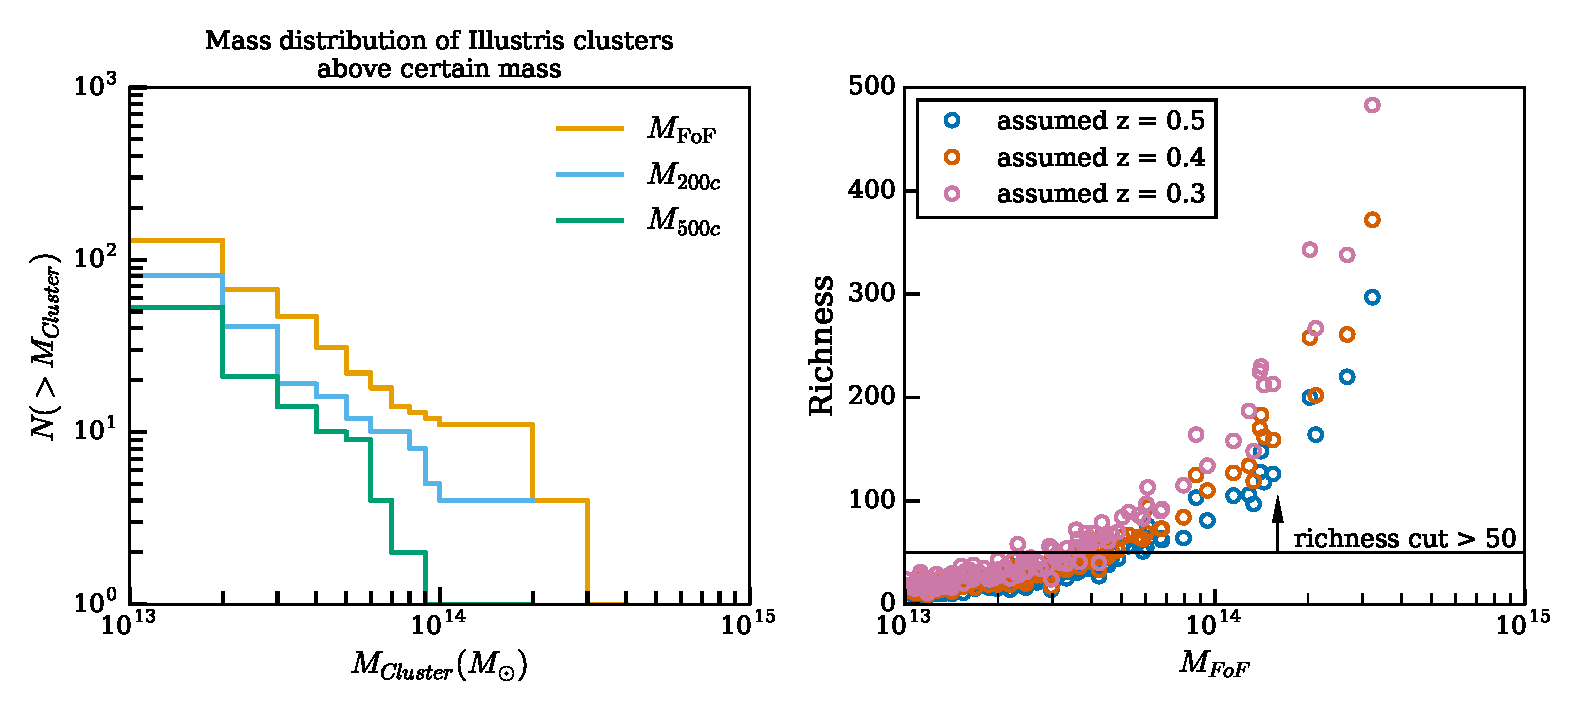
\includegraphics[width=\linewidth]{fig1_mass_richness.eps}
	\caption{ {\bf Left figure:} Mass distribution of the group / cluster sized 
		DM halos for different halo selection schemes. Mass estimates obtained by the
		FoF algorithm are labeled as  M$_{\text{FoF}}$.
		Masses centered on the most bound particle within a radius those the 
		average density is 200 or 500 times the critical density of the universe are 
		labeled as M$_{200c}$ and M$_{500c}$ respectively. 
		% Huge discrepancies between the $M_{500c}$ and $M_{\rm FoF}$ of the clusters 
		% indicate the presence of spatially
		% separated substructures for the clusters (See Fig. 
		% \ref{fig:select_peak_visualization}). 
		{\bf Right figure:} 
		Mass-richness relationship of galaxy clusters and groups with 
		$M_{\rm FoF} > 10^{13} M_{\odot}$ assuming different cosmological redshifts
		of the observed clusters. 
\label{fig:mass_richness}}
\end{figure*}

% Basic setup 
The organization of this paper is as follows:
In section \ref{sec:illustris_sim}, we will describe the physical properties of 
the data of the Illustris
simulation (\citealt{Vogelsberger2014}, \citealt{Genel2014a}), 
and the selection criteria that we have employed to ensure that the
quantities that we examine resemble observables but without noise and
systematics from observations. 
Then in section \ref{sec:methods}, 
we explain the methods for computing various 
one-point statistics of the spatial distribution of galaxies how we prepare our dark
matter spatial data to resemble convergence maps. We show the statistical performance
of the different summary statistics before we show the main results
in section \ref{sec:results}. In the discussion in section \ref{sec:discussion}, 
we list the implications of our
results and compare it to other simulations and observations. We also 
show how one may make use of the population offset statistical distribution
from the Illustris data to construct a test with 
a null hypothesis of $\sigma_{\rm SIDM} = 0$ and discuss the caveats. 

	Our analysis makes use of the same flat Lambda Cold Dark Matter ($\Lambda$CDM) cosmology
as the Illustris simulation. The relevant cosmological parameters are
$\Omega_\Lambda = 0.7274, \Omega_m = 0.2726$, and $H_0 = 70.4$
km~s$^{-1}$~Mpc$^{-1}$.

\section{THE ILLUSTRIS SIMULATION DATA} 
\label{sec:illustris_sim}
The Illustris simulation contains some of the most
realistic, simulated galaxies to date, making it especially suitable for 
verifying the properties of galaxy clusters. We obtained our data from 
snapshot number 135 (cosmological $z=0$) of the Illustris-1 simulation. The Illustris-1
simulation has the highest particle resolution and has incorporated the most 
comprehensive baryonic physics among the different Illustris simulation suites. 
The sophisticated galaxy formation model in Illustris-1 
includes star formation rate, and stellar evolution due to
environmental effects of the intracluster medium, such as ram pressure stripping and
strangulation and feedback from Active Galactic Nuclei (AGN) etc. \citep{Genel2014a}.
The physics of stellar
evolution were solved using a moving mesh code {\bf \texttt{AREPO}} \citep{Springel2010}.
The observable properties of galaxies were statistically consistent
with the Sloan Digital Sky Survey (SDSS) data
\citep{Vogelsberger2014}. 

As the stellar population in Illustris were evolved from the initial condition,
these makes the spatial distribution of galaxies in  Illustris data more 
realistic than galaxies that are prescribed onto DM-only cosmological
simulation data such as those used in \cite{Harvey2013d}.  
Gravitational effects in Illustris-1 have provided realistic dynamics and
spatial distribution of subhalos. The simulated effects include
tidal stripping, dynamical friction and merging. 
Since the profile of the galaxies clusters were not
provided in symmetrical, parametric forms, we can study 
how asymmetry in the cluster profile affects the estimate of our summary 
statistic. This data allows us to examine cluster galaxies
in a realistic, yet noise-free way. The softening length of the DM particles is
1.4 kpc and those of the stellar particles is 
0.7 kpc, both in constant comoving units \citep{Genel2014a}.

The two sets of data catalogs in use are obtained through two types of halo
finders. The catalog that maps particles to the halo of a certain cluster was 
created by the {\bf \texttt{SUBFIND}} algorithm. The friends-of-friends (FoF) 
finder \citep{Davis1985} was further used to identify the affinity
of galaxy-sized halos to a galaxy-cluster. 
These galaxy-size halos are referred to as {\it subhalos} and 
they are the dark matter hosts of what we refer to as galaxies in Illustris-1. 
\cite{Vogelsberger2014a} also extracted the 
absolute magnitude of each subhalo in
the SDSS bands of $g, r, i, z$ as part of the {\bf
\texttt{SUBFIND}} catalog using stellar population synthesis models.

For our analyses, we make use of galaxy clusters / groups 
with at least 50 member galaxies that are within a reasonable observational limit, 
i.e. apparent $i \leq 24.4$ which is the limiting magnitude of the DEIMOS
spectrometer on the Keck telescope when we assume a cosmological redshift of $z = 0.3$
in the $i$ band. The limiting magnitude of 24.2 in the
F814W filter of the Hubble Space Telescope, and the limiting magnitude of the
Canadian-Hawaii French Telescope of 24.5, 
are also close to our chosen limiting magnitude. 
There is relatively large statistical uncertainty if we try
to analyze clusters with less than 50 member galaxies. 
As indicated by the right-hand panel of Fig. \ref{fig:mass_richness}, 
a total of 43 clusters have 
survived this magnitude cut. These simulated galaxy clusters (or groups) have 
masses ranging from $10^{13}$ M$_\odot $ to $10^{14}$ M$_\odot$.  

\begin{figure}
	\centering
	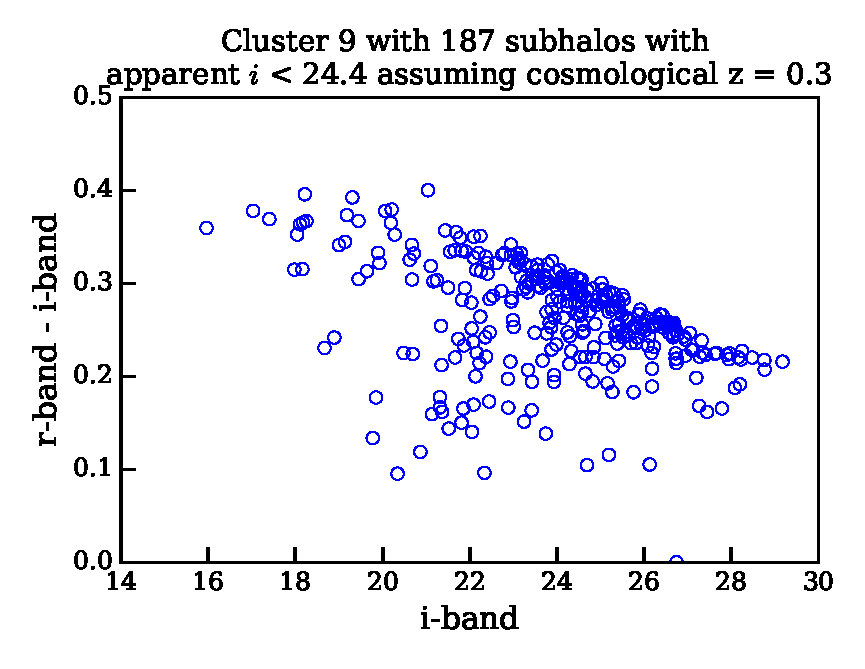
\includegraphics[width=\linewidth]{fig2_color_magnitude_diagram9.eps}
	\caption{Color-magnitude diagram of one of the galaxy clusters that is selected for 
		analysis. This cluster is the 9th most massive. 
		The apparent magnitude is calculated assuming that 
		the cosmological redshift (distance) is $z = 0.3$. 
		We can see a clear overdense region that corresponds to a red-sequence.
		The color-magnitude diagrams of the other clusters can be found in the
		Jupyter notebook at \href{https://github.com/karenyyng/galaxy_DM_offset/blob/master/code/analyses/fig2_color_magnitude_diagram.ipynb}{https://goo.gl/TJmI6s}.
		\label{fig:color_magnitude_diagram}
	} 
\end{figure}

\subsection{Cluster properties}
\label{subsec:cluster_properties}

\subsubsection{Quantifying the dynamical states (relaxedness) of the galaxy clusters}
\label{subsubsec:relaxedness}

Clusters undergo merger activities of a large range of physical scales and 
in the time scale of million of years. 
The dynamical history, or what we call ``unrelaxedness" is hard to retrieve from 
simulations across different saved states and is missing from observations.
We quantify the state of the cluster by providing several quantitative
definitions of unrelaxedness and see how they correlate with $\Delta s$.
Some possible definition of unrelaxedness referred by the simulation community
include:
\begin{itemize}
	\item unrelaxedness$_0$: the ratio of mass outside the dominant dark matter halo over the total mass
		of the galaxy cluster. The lower the ratio, the less substructures there
		are in the cluster. 
	\item unrelaxedness$_1$: the distance between the most bound particle from the center of mass as a
		function of R$_{200c}$, the three-dimensional (3D) radius in which the
		average density is 200 times the critical density of the universe. 
		The smaller the distance, there are less asymmetric 
		substructures. 
	% \item [TODO] velocity dispersion from selected galaxies those selection
	% 	criteria will be explained in  
\end{itemize}
To relate these simulation quantities to observation, 
we compute more observation-oriented 
quantities in the method section \ref{subsubsec:KDE}. 
\subsection{Selection of the field-of-view}
\label{sec:FOV}

\begin{table*}
\begin{center}
\begin{minipage}{180mm} 
	\caption{ Selection criteria for stellar subhalos (member galaxies) for each
		cluster / group 
\label{tab:member_galaxy_selections}} 
	\begin{tabular}{@{}lcccc@{}}
\hline 
Data &  Selection strategy  & Sensitivity & Relevant section  \\ \hline
Field of view (FOV) & FoF halo finder& comparable to FOV of the Subaru
Suprime camera & \ref{sec:FOV}  \\ 
Observed filter & $i$-band & consistent among the redder $r, i, z$ bands &   
\ref{subsec:galaxy_properties}
\\ 
Cluster richness  & $i \leq 24.4$ and $z = 0.3$  & sensitive to
the assumed cosmological redshift of cluster and & \ref{sec:illustris_sim} \\ 
& & the assumed limiting magnitude of telescope &   \\
Two-dimensional projections & even HEALPix samples over half a sphere &
discussed as results  & \ref{subsubsec:projections}\\  
\hline
\end{tabular} 
\footnotesize{
}
\end{minipage}
\end{center} 
\end{table*}

We make use of the {\bf \texttt{SUBFIND}} member particle for the DM and the 
{\bf \texttt{FoF}} subhalo identification as our
default volume selection scheme for each cluster / group.
We understand that this choice of volume selection can be more ideal than
observational conditions. We make use of this volume selection scheme
for baseline comparisons. 

Assuming a conservative line-of-sight (los) distance 
, i.e. cosmological redshift, with [TODO] $z = 0.3$, 
the projected extent for most of the Illustris galaxy clusters and groups, 
fits inside the field of view of telescopes, such as the Subaru Suprime Camera,
which covers a physical area of [TODO] $\sim 9$ Mpc $\times 7$ Mpc 
(See \href{https://goo.gl/ClZNvM}{https://goo.gl/ClZNvM} for a Jupyter notebook 
showing the extent of the Dark Matter distribution of the most massive 129
clusters).

\subsubsection{Spatial Projections}
\label{subsubsec:projections}
Unlike in staged simulation, picking out a particular projection for a cluster 
does not always make physical sense.
For highly symmetrical clusters, most projections are similar. 
However, for mergers or asymmetrical clusters, 
there is no obvious choice for the plane of projection that can allow us to
understand the cluster. There is no simplistic merger axis that should be 
projected along the plane of the field of view due to possible 3D spiraling
trajectories of the merging components. 

We therefore compute observables based on even sampling of angular orientation 
as our line-of-sight.
As the order of projecting the data and estimating the summary statistic is
non-commutative, we first project the data before estimating any projected 
observable. 
The computation of even angular orientation 
is done by using HealPy, which is a Python wrapper for
{\bf \texttt{HEALPix}} \footnote{HEALPix is
currently hosted at http://healpix.sourceforge.net}
\citep{Gorski2005}. Each line-of-sight centers on a {\bf \texttt{HEALPix}} 
pixel.
The number of projections that we employed is 768 for each cluster. With around 
768 projections, the offset distributions of each cluster start to converge to a
stable distribution. 
Even though there are at least 2 identical projections for each cluster due to
one possible line-of-sight from the front and one from the back, it does not
affect any summary statistic. We do not remove the duplication as it breaks
the rotational symmetry in the 2D plane when we try to compute the 2D population
distribution of offsets.  
% Details of the implementation of the projection is available in Appendix
% \ref{app:projections}.


\subsection{Properties of the galaxies in Illustris clusters}
\label{subsec:galaxy_properties}

Different galaxies have different masses, so they should not be considered with equal
importance for peak identification, which requires summing
the mass proxies of different galaxies. One of the most common weighting schemes employed for galaxy data is to weight
by the luminosity in a particular band. For some of the methods, we investigate
the differences in peak identification with and without any luminosity weights.
We pick the $i-$band magnitude
associated with each subhalo as the weight. Since the $i-$band is
one of the redder bands, the mass-to-light ratio is not skewed as much due to star
formation activities. 
We further examined if the colors distribution of galaxies in Illustris-1 are
similar to the observed color-magnitude diagrams for clusters.
The Illustris cluster galaxies are realistic enough that it is easy to
identify an overdense region of galaxies known as the red-sequence in the 
color-magnitude diagram such as Fig.
\ref{fig:color_magnitude_diagram}. The red-sequence is prominent even if we
use other colors formed by different combinations of the $r, i, z$ bands.

\section{METHODS}\label{sec:methods}
A common and the most precise way of summarizing the DM distribution in a
galaxy cluster is by finding the lensing peaks 
(\citealt{Medezinski2013}, \citealt{Markevitch2004}, \citealt{Zitrin13}).
Additionally, the peak region is physically 
interesting due to the higher particle density and interaction rates. 
The most direct analogous statistic for summarizing the member galaxy
population in a cluster is therefore, also the peak. 
Comparing the DM peak with the summary statistics of the galaxy population that
are not the peak therefore can have an {\it offset} purely due to the difference in
the choice of the statistic for summarizing the two sets of identically
distributed data. 
We will state the definition and implementation of five commonly used 
point statistic or location for summarizing 
the member galaxy population in a galaxy cluster.

We avoid any manual methods for
comparison purposes, scalability and reproducibility. 
Since all the methods listed in this
paper are automated with the source code openly available, 
it is possible for future studies to reuse our code for comparisons. 
% There are a number of decisions ($\sim $[TODO] ADD NUMBER) that one needs to make to 
% determine the summary statistics. We will try to address the sensitivity of the offset
% due to each decision. 
Another major advantage for automation is that it allows us  
to apply
the same methods across the different snapshots of the (Illustris) simulations to
examine the variability of $\Delta s$ across time in future studies. 


\subsubsection{Computing the weighted centroid}
\label{subsubsec:weighted_centroid}
We follow the usual definition of the weighted centroid: 
\begin{equation}
	\bar{\bf x}_w = \frac{\sum_i w_i \vec{x}_i}{\sum_i w_i},
\end{equation}
with $\vec{x}_i$ being the positional vector of each subhalo 
and we use the $i$-band luminosity 
as the weight $w_i$ for the $i$-th galaxy.
Centroids can be biased by subcomponents from merging activities yet the
centroid estimate do not provide explicit evidence for ongoing merger or 
accretion. These estimates are also sensitive to odd boundaries 
of the field of view.

\subsubsection{Cross-validated Kernel Density Estimation (KDE) and the peak finder} 
\label{subsubsec:KDE}
Finding the exact peak of a sets of data points 
involves computing the density estimate of the data points and sorting through
the density estimates. A specific version of this density estimation process is
known as histogramming. During the making of histogram, each data point is
given some weight using a tophat kernel and the weights are summed up at
specific data locations (e.g. $\bf{x}_i$). 
Histogram is not good for peak estimate for {\it sparse} data for two reasons: 1) the
choice of laying down the bin boundaries affects the count in each bin, 2) the choice of
bin width also affects the count in the bin. Only when the available number of data points
for binning is large, the estimates of histograms and smoothed density
estimates are approximately the same. The number of member galaxies ($< 500$) 
is sparse enough for the uncertainty introduced by histogramming to bias our
peak estimate. For the density estimate of galaxy luminosity, 
we adopt a Gaussian kernel. 
The exact choice of the functional form of the smoothing kernel does
not dominate the density estimate as long as the chosen kernel is
smooth \citep{Feigelson2014}. 

For computing the density estimate, the most important parameter of computing 
is the bandwidth of the smoothing kernel, 
which takes the form of a matrix in the 2D case. 
 We illustrate the choice of kernel width with Fig.
\ref{fig:bias_variance_tradeoff}. When the kernel width is
too large (bottom left panel), the data is over-smoothed, 
resulting in a bias of the peak estimate. On the other hand, when the kernel
width is too small, it results in high variances of the estimate and result in
too many peaks due to noise. The decision of having to balance between creating high
bias or high variance estimates is also known as the bias-variance tradeoff. 
Any other smoothing procedures, including interpolation with splines,
polynomials, and filter convolutions, also face the same tradeoff. 

\begin{figure*}
	% \includegraphics[width=\linewidth]{figN_mass_richness.eps}
	\caption{This figure is adapted from \citealt{Vanderplas2012} from
\href{http://www.astroml.org/book\_figures/chapter6/fig\_hist\_to\_kernel.html}{http://www.astroml.org/book\_figures/chapter6/fig\_hist\_to\_kernel.html}
under the fair use of the BSD license. \label{fig:bias_variance_tradeoff} }
\end{figure*}
A well-known way to minimize the fitting error from the density estimate is through
a data-based approach called cross-validation to obtain 
the optimal 2D smoothing
bandwidth matrix ($\Hmat$) of the 2D Gaussian kernel for the
density estimate $\hat{f}$:
\begin{align}
	\hat{f}(\chi; \Hmat) &= \frac{1}{n} \frac{1}{(2\pi)^{d/2}|\Hmat|^{1/2}}
	\sum_{i=1}^n w_i \exp((\chi-{\bf x}_i)^T H^{-1} (\chi-{\bf x}_i)),
	\label{eq:cross_validated_bandwidth}
\end{align}
where the dimensionality is $d=2$ for our projected quantities,
$\chi$ represents the uniform grid points for evaluation, and 
$\bf{x}_i$ contains the spatial coordinates for each of the identified member 
galaxies that survived our brightness cut and $w_i$ is again the $i-$band
luminosity weights for each galaxy.
The idea behind cross-validation is to leave a small fraction of data point 
out as the test set, and use the rest of the data points as 
the training set for computing the estimated density.
Then it is possible to estimate and minimize the asymptotic mean-integrated squared error
(AMISE)  by searching
for the best set of bandwidth matrix values, eliminating any free parameter. 

Specifically, we made use of the smoothed-cross validation \citep{Hall1992} 
bandwidth selector in the statistical package {\bf \texttt{ks}} \citep{Duong2007} 
in the {\bf \texttt{R}} statistical computing environment \citep{R_core}. 
Among all the different {\bf \texttt{R}} packages, {\bf \texttt{ks}} is the
only package capable of handling the magnitude weights of the data points 
while inferring the density estimates \citep{Deng2011}. 
Although the particular implementation of KDE has a computational runtime of $O(n^2)$, 
the number of cluster galaxies is
small enough for this method to finish quickly ($\lesssim 2$ second per
projection per cluster). 

The resulting KDE contains rich information about the spatial distribution of
the clusters, and we focus on the peak regions.  
We employed both a first and second-order  
finite differencing algorithm to find the local maxima.  
The local maxima were then sorted according to the KDE density in a descending
fashion before we perform peak matching and compute the offset. The exact
procedure is discussed in section \ref{subsec:offsets}. 

The number of distinct subclusters are also occupied by a bright peak.
For each projection of each cluster, we normalize the density of all 
luminosity peaks to those of the brightest peak. 
Then we sum the density of all the galaxy peaks for a cluster and call this value
$\nu$. When the value of $\nu$ much gets bigger than 1, it indicates the presence 
of projected substructure(s). Even though 
$\nu$ is not expressed in terms of masses, it is a practical measurement
for optical survey data where only galaxy magnitudes, but not spatial mass distribution 
from lensing estimates, are available. 
% Another possible quantification of relaxedness can be computed based on the
% (morphology) ratio of eigenvalues of the galaxy luminosity map bandwidth matrix. 

\subsubsection{Shrinking aperture estimates}

Another popular method among astronomers for finding the peak of a spatial
distribution is what we call the shrinking aperture method.
While we do not endorse this method,
we test if the shrinking aperture method is able to reliably recover the 
peak of the luminosity map.
This method is dependent on the initial diameter and the initial center 
location of the aperture.
This method does not evaluate if the cluster is made up of
several components.
The estimate using the shrinking aperture algorithm can be biased by
substructures. The only way to inform the algorithm about substructures would
be to introduce another parameter to restrict the extent of the aperture, or to
partition the data with another (statistical) algorithm.
More to the point, the convergence of results of this method is unstable. We use a
convergence criteria of having the aperture distance not change more than 2\% 
between successive iterations as a reference. The actual implementation in
Python can be found at \href{https://goo.gl/nqxJl8}{https://goo.gl/nqxJl8} while
the pseudo-code can be find in Appendix \ref{app:shrink_apert}.

\subsubsection{Brightest Cluster Galaxies (BCG)}
The BCGs are formed by the merger of many smaller
galaxies. The galaxy-cannibalism makes BCGs typically brighter than the rest of 
the cluster galaxy population by several orders of magnitude. 
However, star formation can cause
less massive galaxies to be brighter in the bluer photometric bands.
To avoid star formation from biasing our algorithm for identifying the
BCG, we find the brightest galaxies in redder bands i.e. the $r, i, z$
bands and found that they give consistent results for all selected clusters. 
We used the $i-$band to pick the BCG for computing the plots and the final results. 
 
\begin{figure*}
	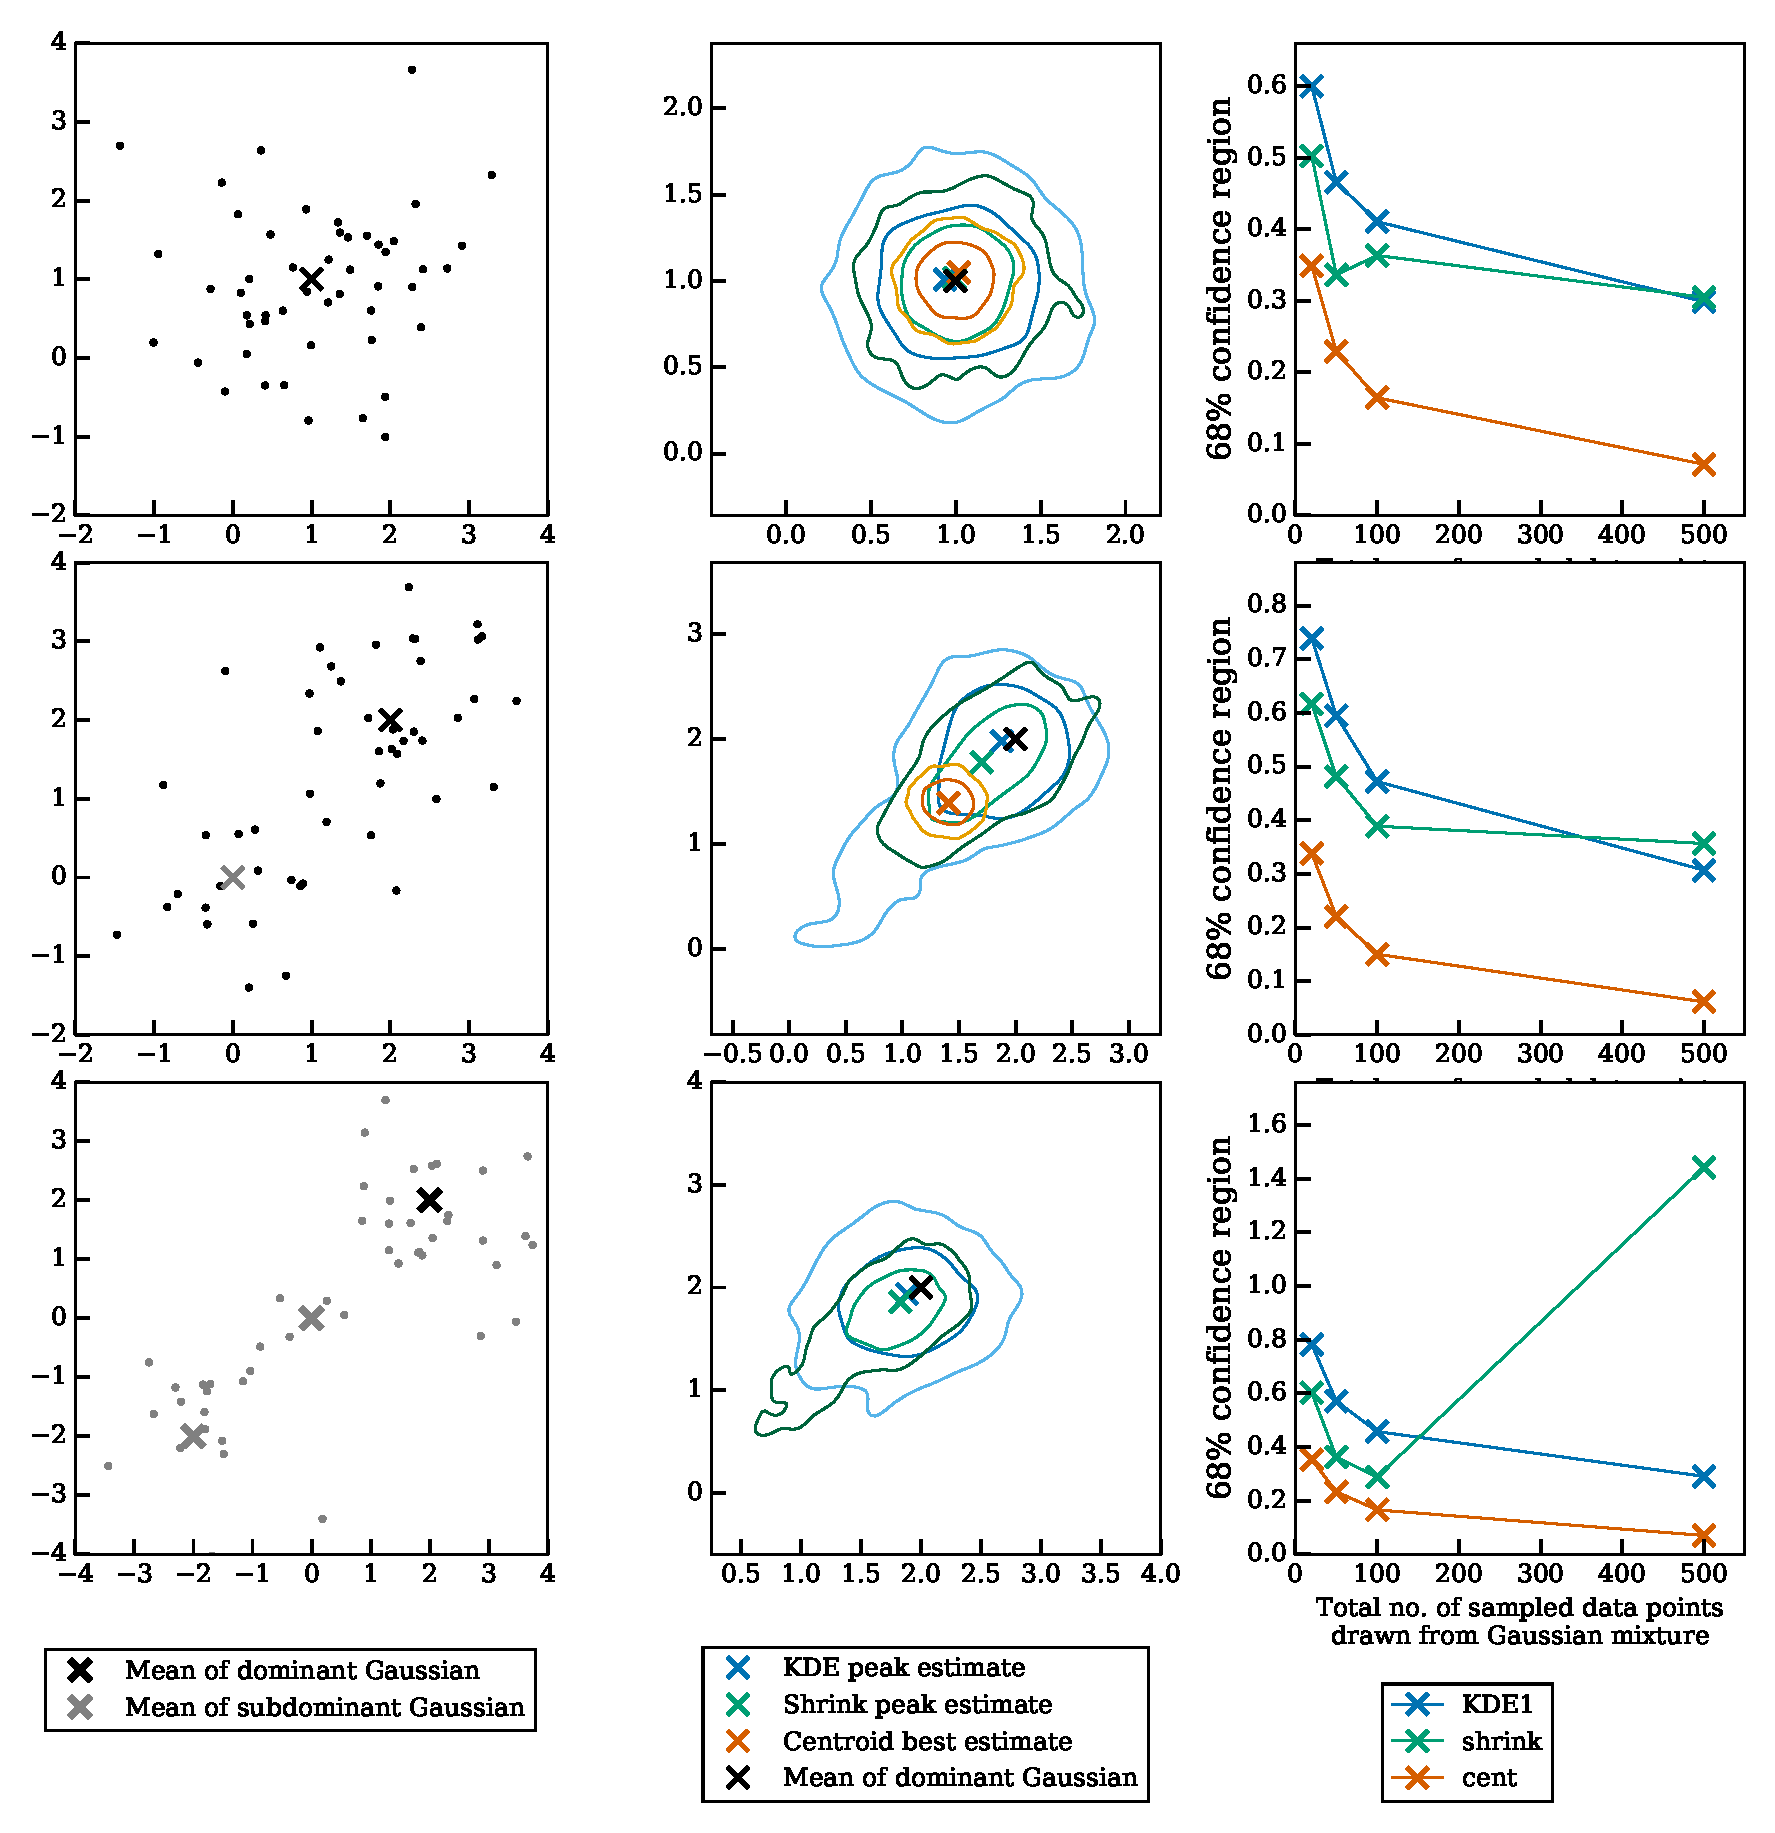
\includegraphics[width=.95\linewidth]{fig3_toy_data_mixtures.eps}
	\caption{Comparison of peak finding performances of different methods by
		drawing data points (i.e. 20, 50, 100, 500) from known number of 
		Gaussian mixtures. 
		Panels from the top row contain data drawn from a single Gaussian mixture. The
		panels from the middle row contain data from two 
		 Gaussian mixtures with weight ratio = 7:3. 
	The panels from the bottom row contain data drawn from three Gaussian
	mixtures with weight ratio = 55:35:10. 
	The left column shows how 50 data points drawn from the fixed number of 
	Gaussian mixtures look like. 
	Due to the statistical nature of this exercise, we sampled the data and
	performed the analyses [TODO: state how many times] many times to
	create the 68\% and 95\% Monte Carlo confidence contours of the estimates in the
	zoomed-in view of the data in the middle
	column. The rightmost column shows how the size (median contour radius) 
	of the confidence regions vary as a
	function of the number of drawn data points from the Gaussian mixtures. 
	From the middle and the rightmost
	column, we can tell that the KDE peak estimate is the most accurate. [TODO] 
		\label{fig:toy_data_mixtures}}
\end{figure*}



\subsection{Comparison of the methods from Gaussian mixture data}
In order to examine the statistical properties of commonly used point-
estimates of the distribution of the galaxy data, we test them on data drawn 
from Gaussian mixtures with known mean and variance. (See Fig.
\ref{fig:toy_data_mixtures}). The main factors that affect the performance of 
the methods are sensitive to the statistical fluctuations of the drawn data, 
e.g. the
spatial distribution of the data, including 1) the density profile and 2) the
location(s) of subdominant mixtures,
, and 3) the number of data points that we draw.
It is also not enough to just
compare the performance by applying each method for one realization of the
data. We provide the 68\% and the 95\% confidence regions by applying the
each method for many Monte Carlo realizations.
In general, the peaks identified from the KDE density is closer to the 
peak of the dominant mixture (more accurate) than 
both the weighted centroid method and the shrinking aperture method.
For example, in the bottom middle panel of fig. \ref{fig:toy_data_mixtures}, 
it is clear that the green contours
that represents the confidence region for the shrinking aperture peak is
biased due to the substructure, whereas the confidence region for the centroid 
is so biased that it is outside the field of view of that panel.
For the bottom right panel of fig. \ref{fig:toy_data_mixtures}, 
we present how the confidence region shrinks as the
number of data points increases.
From that here is also a catastrophic outlier for the shrinking 
aperture method for 500 data
points. The outlier shows how the shrinking aperture method can have
radical behavior when there are subclusters in the data.	

\subsection{Modeling the DM map in Illustris-1 and the lensing kernel}
The most well established method of inferring the projected dark matter spatial 
distribution from observations is through gravitational lensing.
It works by detecting subtle image distortions of background galaxies due to
the foreground dark matter. The resolution of the inferred map therefore 
depends on the properties of the source galaxies that are being lensed, 
such as the projected number density, the intrinsic ellipticities and morphology etc.
To achieve a sufficient signal-to-noise ratio for lensing, 
\cite{Hoag2016} has performed simulation for inferring the optimal bandwidth
for a Gaussian smoothing kernel for the cluster MACSJ0416. 
In the strong lensing regime, \cite{Hoag2016} found a resolution of 11 arcseconds
can best fit the MACSJ0416 data. A kernel bandwidth (this is the standard deviation) 
of 11 arcseconds translates to an angular diameter distance of 50 
kpc assuming a cosmological redshift of $z \approx 0.3$. 
\cite{Clowe2012} also described using a 60 kpc radial Gaussian kernel to smooth out spikes
in the weak lensing map of Abell 520. In order to match the resolution of lensing data,
we also employed a smoothing kernel of a similar physical size of 50 kpc.  

To compute the DM spatial distribution from our data, we first make histogram with 2 kpc
$\times$ 2 kpc bin size which is slightly larger than the DM softening length of 1.4 kpc. 
After that, we use a (50, 50) kpc 2D radial Gaussian kernel 
to smooth the DM histogram Illustris DM
particle data. 
There are resolution differences between the smoothed and unsmoothed DM
maps. The unsmoothed histograms tend to show many more local maxima around the major
density peaks (i.e. show high variance). 
The number of DM particles for each cluster is of 
[TODO double check] the order of millions and densely packed in the region of
interest. 
Physically, the smoothed histograms of the dark matter of each cluster 
is analogous to a convergence map from a lensing analysis. 


\subsection{Finding the offsets} \label{subsec:offsets}
It is possible to have several peak estimates from the KDE of the member galaxy 
population of a cluster. 
From the density estimate at each peak, we can sort 
the peaks according to their densities. We only match luminosity 
peaks that are at 
least 20\% as dense as the brightest galaxy-luminosity peak to avoid 
computing the offsets of spurious substructures, such as the peaks due to 
small number of galaxies that are located far away from the main concentration of mass.

In general, there are many more DM peaks because there are many more dark 
subhalos than galaxies for each cluster and the resolution of the DM data is
much higher. To find the nearest DM peak to the significant galaxy peaks just as any
astronomers would do manually,  
we construct a k-dimensional tree (KD-Tree; in our case, k = 2) 
using the densest $n_{\rm DM}$  number of DM peaks:
\begin{equation}
	n_{\rm DM} = \begin{cases}		
		3 \times (n_{gal} + 1) & {\rm if~} n_{gal} < 3 \\
	3 \times n_{gal}  & {\rm if~} n_{gal} \geq 3.
	\end{cases}
	\label{eq:peak_threshold}
\end{equation}
where $n_{gal}$ is the number of significant galaxy peak, and $n_{\rm DM}$
is the number of peaks that went into the construction of the KD-tree.
When there are more
than one dense galaxy peaks located far away from one another, 
the top few densest DM peaks (subhalos) 
can be located around the same galaxy peak.
i.e. there is no one-to-one matching between the luminosity of galaxies and the
density of detected DM peaks.
Matching purely based on density and luminosity leads to larger offsets.
From inspection, using eq. (\ref{eq:peak_threshold}) works well to match the 
appropriate peaks. We also show in the result section that most of the chosen DM peaks
do not have significant deviation from the most gravitationally bound particles.
After identifying the DM peaks, we also compute the 
offsets 
between the DM peaks, and the following spatial estimates, including 
\begin{itemize}
	\item the most (gravitationally) bound particle 
	\item the shrinking aperture peaks, the corresponding offset is $\Delta s_{\rm
		shrink}$, 
	\item the number density peaks, the corresponding offset is $\Delta s_{\rm
		num.dens}$, 
	\item the BCGs, the corresponding offset is $\Delta s_{\rm BCG}$ and
\item the luminosity weighted centroid, the corresponding offset is $\Delta s_{\rm BCG}$.
\end{itemize}
Since there can be more than one number density peak from the corresponding KDE
map, we also use a KD-tree to location the closest number density peak to the 
identified DM peak.

[TODO] Figure out how the Illustris simulation figure out the most bound 
particle.
The most bound particle is the location with minimum 
gravitational potential of the {\bf \texttt{Subfind}} identified cluster.
Due to substructures, it is possible for there to be several minima of similar 
gravitational potential level. 

\subsection{Constructing the hypothesis test} 

After matching the peaks, we use the offsets as the basis of our 
 hypothesis test. 
We compute the p-value as the narrowest density interval of simulated offsets 
that are below observed values of 
offsets in the literature. The distribution of offsets in the Illustris
simulation represents the possible ways that offsets would be observed in a CDM
universe.
This gives us a rough estimation of the probability 
of seeing the offset from observations under the null hypothesis of CDM 
being true. We also provide the biweight location and the density interval 
characterizing the 
distribution of offsets computed from each of the listed methods.
For instance, the 95\% interval is computed as the interval that encompasses
95\% of total density (2.5\% of density mass at each end of the tail is
excluded). In case of degeneracy, the interval is also required to cover the 
location estimate for the distribution.

The different representations of the distributions of $\Delta s$ have different 
statistical power for the hypothesis test, i.e. there are discrepancies between
the spread of the offset distributions, so
it affects the significance of an observation. 
The most faithful representation of the offsets without any information loss
is:
\begin{equation}
	\Delta {\bf s} = ({\bf x}_{\rm gal} - {\bf x}_{\rm DM}, 
	{\bf y}_{\rm gal} - {\bf y}_{\rm DM} ).
	\label{eq:2D_offsets}
\end{equation}
The PDF of $\Delta {\bf s}$ in eq. \ref{eq:2D_offsets} peaks at (0, 0) when there is no real offset.
However, when one takes the magnitude of $\Delta {\bf s}$, i.e.:
\begin{equation}
	|\Delta {\bf s}| = \sqrt{({\bf x}_{\rm gal} - {\bf x}_{\rm DM})^2 + 
	({\bf y}_{\rm gal} - {\bf y}_{\rm DM})^2},
	\label{eq:magnitude_offsets}
\end{equation}
the resulting 1D distribution of $|\Delta {\bf s}|$, 
those support being [0, $\infty$),
will not peak at zero even if the original
distribution of $\Delta {\bf s}$ peaks at (0, 0). 
To illustrate how difficult it is to interpret the magnitude values $|\Delta
s|$,  
we can imagine the following transformation.
The values drawn from: 
\begin{equation}
	\left(\begin{array}{c}
			\bf{x}\\
			\bf{y}
		\end{array}
	\right) \sim \mathcal{N}\left(
	\left(
		\begin{array}{c}
			0 \\
			0
		\end{array}
	\right),
	\left(\begin{array}{cc}
		\sigma^2, 0 \\
		0, \sigma^2
	 \end{array}
	\right)
\right),
\end{equation}
will result in $|\Delta s|$ values that follow the Rayleigh distribution:
\begin{equation}
	f(\Delta s | \sigma) = \Delta s /  \sigma^2 \exp(-\Delta s^2 / 2 \sigma^2)
\end{equation}
those peak is at $|\Delta s| = \sigma$, the standard deviation of the 2D
Gaussian and 
ruling out any probability mass at $|\Delta s|$ = 0 by construction. 
The dependency of $|\Delta s|$ on the parameters of
the 2D distribution is even more
complicated when the the 2D distribution does not approximate a Gaussian 
or when there is more than one peak in the 2D space. 
The shifting of the peak location due to variable transformation 
is seen in the distribution of $|\Delta {\bf s}|$ recorded in table
\ref{tab:offset_distributions}.
For an asymmetrical 1D distribution due to taking the magnitude, 
finding the narrowest 68\% and 95\% interval
is not a standard statistical procedure and can be prone to error.
In fact, several studies have reported poor single 2D Gaussian fits to 2D offset data
due to the long tails
(\citealt{Zitrin2012a}, \citealt{Oguri2010}).  

On the other hand, 
the 1D distributions of offsets along a particular spatial axis, 
e.g. $\Delta {\bf x}$ and $\Delta {\bf y}$,
each with a support of $\mathbb{R}$, will not exhibit a discontinuity at zero.
Any shift in the 2D peak location is still obvious. 
The distributions represented by $\Delta x$ or $\Delta y$ 
can be symmetrical without any sharp cutoff at zero so 
the highest density interval is easier to find.
Since we have enough samples for there to be
rotational symmetry for the distribution of $(\Delta {\bf x}, \Delta {\bf y})$,
we will show that it does not
matter much if we picked $\Delta {\bf x}$ or $\Delta {\bf y}$ for the 1D representation.
We compute the hypothesis test significance level with the 
 offset $\Delta {\bf x}$ along one of the spatial axes. 
To report the statistics, we also make use of estimates that do not make any
underlying assumption of the shape of the distributions that may skew the
statistical parameter estimate.
We report the percentile for the offset distributions, and also the biweight 
statistical estimates such as the biweight 
location (analogous to the median)
and the midvariance (robust standard deviation
estimate). The biweight statistics are less susceptible to the effects of
outliers \citep{Beers90}. We compute the robust statistics using the implementation
from \cite{astropy} as part of {\bf \texttt{astropy}}. 

In following sections of this paper, we use $\Delta {\bf s}$  to represent the
two-dimensional offsets, $|\Delta {\bf s}|$ for the magnitude of the offset as calculated
according to the Euclidean distance, and $\Delta x$ or $\Delta y$ to denote the
one-dimensional offset along one of the spatial dimensions.
To compare with observed data, we estimate the 1D spatial components of
the offsets from the merging cluster observations from various sources.   
We make our best attempt to measure $\Delta y_{\rm obs}$, the spatial component of the
observed offset along the axis connecting the subclusters if subcomponents exist. 
In our observed samples, Abell 3827 is the only exception to have no
subclusters but only four bright galaxy peaks in the central region. 
We also show $\Delta x_{\rm obs}$ components, the offset perpendicular to
$\Delta y_{\rm obs}$ for comparison.
For most of the observed offsets, we obtain the estimates from the contour plots 
and descriptions of the corresponding papers. 
For the offsets that are roughly in line with the axis connecting the two subclusters,
we let $\Delta y = |\Delta {\bf s}|$. 
If $\Delta s_{\rm obs}$ is not aligned along the line joining the subclusters,
using $|\Delta s_{\rm obs}|$ instead of $\Delta y_{\rm obs}$ to come 
up with a p-value from the distribution of 
$\Delta y$ will lead to an spurious increase in significance.


% There is a more comprehensive discussion of the representation of offset 
% distributions and the complications due to the different projections of the
% clusters in Appendix [TODO]. 
 
\section{RESULTS} 
\label{sec:results}

\begin{table*}
	\begin{minipage}{170mm}
	\begin{center}
		\caption{Robust estimates and the distribution of offsets along the y-axis
			(This is different from the magnitude which has discontinuity at zero).
		\label{tab:p_val_table}
	}
	\begin{tabular}{llccccccc}
\toprule
sample & offset (kpc  &  location &  lower 68\% &  lower 95\% &  lower 99\% &  upper 68\% &  upper 95\% &  upper 99\% \\
\midrule
all $\nu$& $\Delta y_{\rm BCG}$                &         0 &          -3 &         -22 &        -496 &           3 &         456 &        1449 \\
& $\Delta y_{\rm KDE}'$               &         0 &         -25 &         -79 &        -127 &          25 &          79 &         126 \\
& $\Delta y_{\rm num. dens}$          &        0 &         -84 &        -303 &        -693 &          84 &         302 &         691 \\
& $\Delta y_{\rm shrink}'$            &        0 &         -65 &        -295 &        -652 &          65 &         295 &         655 \\
\midrule
$\nu < 1.2$& $\Delta y_{\rm BCG}$              &        0 &          -3 &         -10 &         -19 &           2 &           9 &          19 \\
& $\Delta y_{\rm KDE}'$             &         0 &         -18 &         -48 &         -82 &          18 &          48 &          83 \\
& $\Delta y_{\rm centroid}'$         &        0 &        -108 &        -255 &        -395 &         108 &         254 &         394 \\
& $\Delta y_{\rm num. dens}$        &        0 &         -73 &        -195 &        -303 &          73 &         195 &         302 \\
& $\Delta y_{\rm shrink}'$          &         0 &         -51 &        -187 &        -285 &          51 &         187 &         285 \\
\midrule
$1.2 < \nu < 2.0$& $\Delta y_{\rm BCG}$        &         0 &          -3 &        -172 &        -699 &           4 &         860 &        1597 \\
& $\Delta y_{\rm KDE}'$       &        0 &         -33 &         -90 &        -128 &          33 &          90 &         127 \\
& $\Delta y_{\rm centroid}'$   &         0 &        -266 &        -673 &        -926 &         266 &         673 &         926 \\
& $\Delta y_{\rm num. dens}$  &         0 &         -89 &        -350 &        -776 &          89 &         347 &         776 \\
& $\Delta y_{\rm shrink}'$    &        0 &         -85 &        -385 &        -773 &          85 &         385 &         776 \\
\bottomrule
\end{tabular}

	\end{center}
	\end{minipage}
\end{table*}

% \begin{landscape}
\begin{table*}
	% \begin{minipage}{180mm} 
	\centering
	 \caption{Observed offsets from clusters with reported evidence of mergers
		 along line connecting two subclusters ($\Delta y$) and the approximate 
		 perpendicular offset ($\Delta$ x).
		 The table mainly contains clusters that have been used to constrain
		 $\sigma_{\rm SIDM}$ using the reported offsets.
	 Any approximate  
	 error estimates are the corresponding 68\% lensing peak uncertainty
	 in the figure(s) of the references, this is due to the lack of uncertainty
	 estimates from the galaxy summary statistics from most literature. 
		Error estimates are omitted when they are not reported by the authors.  
	 All p-value lower bounds are reported by matching to the corresponding method for
	 estimating galaxy summary statistic in table \ref{tab:p_val_table}.
	 \label{tab:offset_results}} 
	 \begin{tabular}{@{}lccccccccc@{}}
	 \hline 
	 Cluster &$\Delta y$ (kpc) & $\Delta x$ (kpc) & $|\Delta s|$ (kpc) & galaxy peak & DM peak &  p-value & subcluster &
	 mass ($10^{14}$ M$_\odot$)  &  reference\\
	 \hline
	 Bullet  & 9  & -23 & 25$~\pm~29$ & num. or lum. & SL \& WL & $\gtrsim 0.32$ &
	 northwest & 1.5 & \citealt{Randall2008d}\\
	 Baby Bullet & -40&  0 & $\sim 40 \pm \sim 50 $  & lum. & SL \& WL &
	 $\gtrsim 0.05 $ & northwest & 2.6 &
	 \citealt{Bradac2008}:Fig.4 \\
	 Baby Bullet & 30  & 0 & $\sim 30 \pm \sim 75 $ & lum. & & $\gtrsim
	 0.32 $&
	 southeast
	  & 2.5 & \citealt{Bradac2008}:Fig.4 \\
	 Musketball &  129 & 0 & 129 $\pm \sim 63$ & num. & WL & $>0.05$ &
	southern & 3.1 
	 & \citealt{Dawson2013}:Fig.4.7\\
	 Musketball & -47 & 0 & 47 $\pm \sim 50$ & num. & & $>0.32$ &
	 northern & 1.7 &  
	  \citealt{Dawson2013}:Fig.4.7\\
		Abell 3827 & 6 & 0 & 6 & BCG & SL & $> 0.05$ & central & & \citealt{Williams2011a}\\ 
		Abell 520 & 0 & 50& $\sim 50 \pm \sim 50$ & lum. & WL & $\gtrsim 0.32$ & blue 
		 & 5.7 & \citealt{Clowe2012}:Fig. 4 \\
	 % Abell 1689  & & & & & &  & \citealt{Mohammed2014} \\
		El Gordo &  58 &0 & $\sim 58 \pm \sim 100$ & lum. & WL & $>0.05$ & 
		northwest& 11  &\citealt{Jee2014}:Fig.7,8  \\
		El Gordo & 30 & 110 & $ 115 \pm \sim 60$ & num. & & $>0.32$ & 
		northwest&   &\citealt{Jee2014}:Fig.7,8  \\
		El Gordo & 6 & 25& $\sim 26 \pm \sim 50$ & lum. & & $>0.32$ & northwest & 7.9   
		&\citealt{Jee2014}:Fig.7, 8  \\
		El Gordo & 280 & 280 & 400 $\pm \sim 40$ & num. & & $>0.05$ &
		southeast &   &\citealt{Jee2014}:Fig.7, 8  \\
		Sausage &160 & 100& $\sim 190\pm \sim 150$ & num. & WL & $\gtrsim
		0.05$ & north & 11.  &\citealt{Jee2015}:Fig.10\\ 
		Sausage &160 & 160& $ \sim 190\pm \sim 150 $  & num. &  & $\gtrsim
		0.05$ & south & 9.8 & \citealt{Jee2015}:Fig.10\\ 

		Sausage & 320 & 130 & $\sim340 \pm \sim 150 $  & lum. & & $\lesssim
		0.01$ & north & 11. & \citealt{Jee2015}:Fig.10\\ 

		Sausage & 160 & 160 &$\sim230 \pm \sim 150 $  & lum. & & $\lesssim
		0.01$ & south & 9.8 &\citealt{Jee2015}:Fig.10\\ 
	 \hline
	 \end{tabular} 
	 \raggedright{
		 {\it num.} is a short hand for the peak estimate from the number
		 density map. \\
		 {\it lum.} is a short hand for the peak estimate from the luminosity
		 density map, or KDE' in the method description. \\
		 {\it SL} is a short hand for strong lensing. \\
		 {\it WL} is a short hand for weak lensing. \\
	 }

\end{table*}
% \end{landscape}


\begin{figure*}
	\begin{center}
	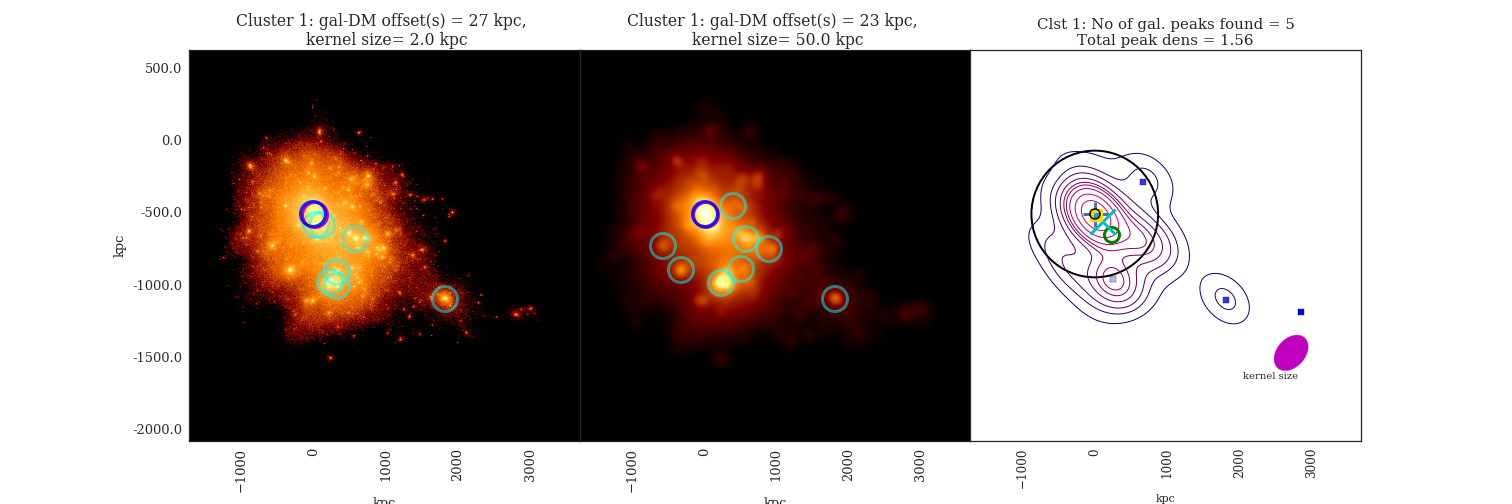
\includegraphics[width=0.85\linewidth]{Fig4_clst1_48_225.png}
	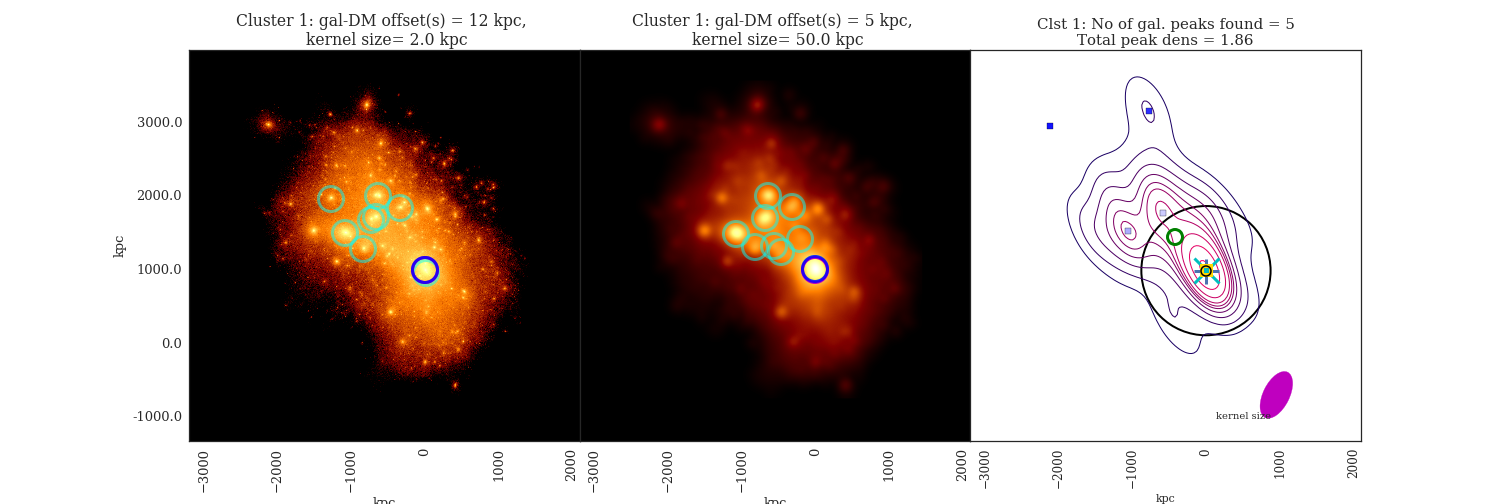
\includegraphics[width=0.85\linewidth]{Fig4_clst1_48_135.png}
	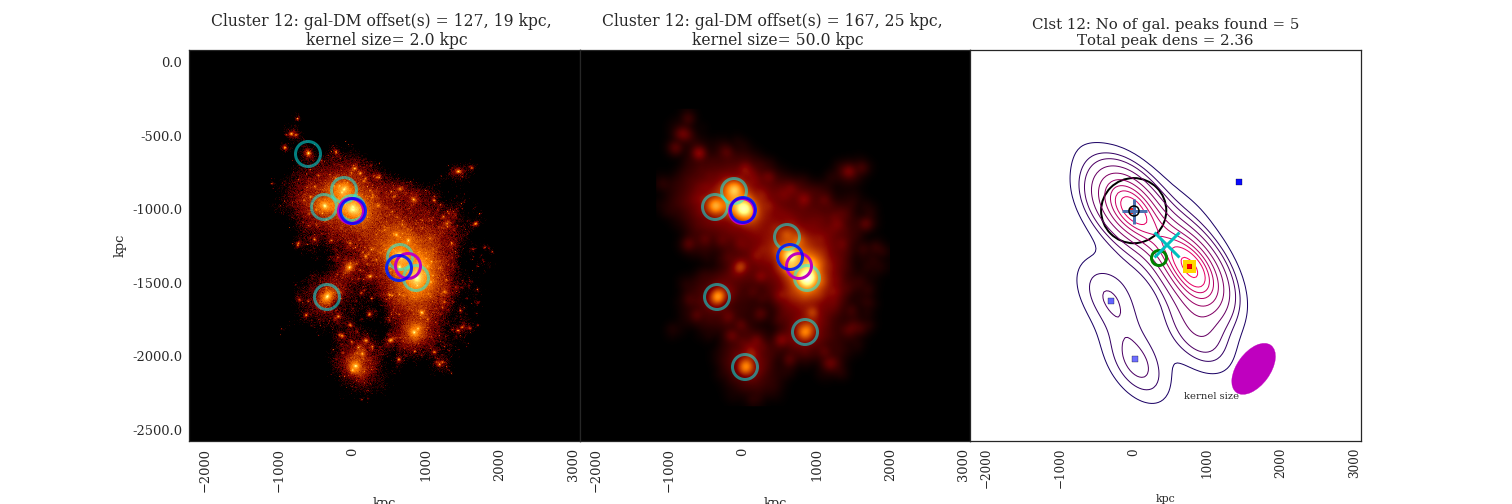
\includegraphics[width=0.85\linewidth]{Fig4_clst12_48_135.png}
	\caption{	Visualization of clusters (each row is for the same projection
		of the same cluster). {\bf Left column:} Projected density distribution of DM	
		particle data is shown in orange, with the dense regions in yellow. 
		The identified density peaks are indicated by colored circles. 
		{\bf Middle column:} The same DM projection after smoothing with a 50 
		kpc smoothing kernel (kernel size is indicated by a white dot on lower right of
		the panel. The thickness of the dot may be larger than 2 kpc
		for the plots on left hand column).
		{\bf Right column:} Projected galaxy kernel density estimates (KDE) of 
		the $i$-band luminosity map for the member
		galaxies of the same clusters. Each colored contour denotes a 10\% drop 
		in density mass starting from the highest level in red. Each of 
		the magenta ellipse on the
		bottom right corner of each plot show the Gaussian kernel matrix 
		$H$ from eq. (\ref{eq:cross_validated_bandwidth}). 
		The big black 
		circle is centered on the most bound particle as identified by {\bf
		\texttt{SUBFIND}} and the radius of the circle indicates the 
		R$_{\rm 200C}$. The luminosity peaks (square markers) are colored
		by the relative density to the densest peak, the relative density  
		is shown by the color bar.  
		See \href{http://goo.gl/WiDijQ}{http://goo.gl/WiDijQ} 
		and \href{http://goo.gl/89edcM}{http://goo.gl/89edcM} for the 
		visualization of the selected clusters inside two Jupyter notebooks.
		\label{fig:select_peak_visualization}
	}
\end{center}
\end{figure*}

\subsection{The dynamical states (relaxedness) of the clusters}
Out of the $43 \times 768 = 33 024$ projections, $\sim 45\%$ of the projections 
have one dominant luminosity peak and negligible substructures, with the total peak density of the
projection being $\nu \leq 1.2$. 
Another $\sim 50\%$ of the projections have more than one dominant luminosity
peak with $1.2 < \nu < 2.2$. 
From Fig. \ref{fig:total_peak_dens_distribution} that shows the spread of $\nu$
estimate over different projections, 
most clusters show signs of other subdominant peaks.

Visually, the spread of the $\nu$ distribution is indicated by the horizontal 
length of the blue box. 
the median of $\nu$ per cluster are indicated by the red central vertical line
inside each box in Fig. 
\ref{fig:total_peak_dens_distribution}.
Only 7 clusters (with ID = 15, 16, 17, 22, 31, 35, 51) out of 43 clusters have $\nu
\lesssim 1.2$ for most of the projections.
Clusters with median values of $\nu > 2.2$ usually have multiple subclusters.
Cluster with ID = 7, for instance, is made up of around 4 disconnected clusters that span
several Mpc.  
There is also a strong correlation of $\sim 0.8$ 
between each of the two unrelaxedness quantities defined in section 
\ref{subsubsec:relaxedness}
and the median of $\nu$ over different projections of each cluster. 


\subsection{Offset between the matched DM peaks and the corresponding most
bound particle}
There is no significant differences between the matched DM peaks and 
the most gravitationally 
bound particle (hereafter most bound particle).
The median of the offset between the DM peak and the gravitationally bound
particle is (0, 0) kpc. The 75-th percentile of the offsets are at ($\pm2,\pm2$) kpc. 
Most of the other offset values occur below ($\pm 9, \pm 9$). Large offsets
are only seen for clusters with $\nu > 1.2$. The densest DM peak in 3D where
the most bound particle is located, does not
necessarily correspond the densest projected peak in 2D in the presence of 
significant DM substructures.   

\subsection{Offset between galaxy summary statistic and the most bound particle}
As another sanity check, we computed the offsets between different galaxy summary
statistic and the most bound particle. 
Interested reader can refer to table
\ref{tab:most_bound_particle_offset_distributions} for the different
percentile and robust estimates of the distribution of offsets from the most bound 
particle. 
The ranking in terms of increasing distance 
to the most bound particle computed by different method is as follows:
\begin{itemize}
	\item BCG 
	\item densest peak of the luminosity map created by weighted the KDE 
		\item shrinking aperture center from the luminosity weighted galaxy data
		\item densest peak of the number density map created by the unweighted KDE 
		\item centroid estimate using luminosity weights, which is a proxy for the
			center of mass
\end{itemize}

In fact, most of the BCG offsets are very small except for two clusters with ID 13
and 33. Both clusters have all the values  of $\nu > 1.5 $ over different projections. 
From the projected density map, we further confirm that
both clusters have significant substructures. It is therefore possible for the
most bound particle to have similar gravitational potential level as another 
substructure where the BCG is located. 
In general, the offset distributions between the galaxy summary statistics and
the most bound particle have approximately the same level of variance but more
extreme outliers (at the 99\%) than the
offset distribution between the DM peaks and the corresponding galaxy summary
statistics.

\subsection{Galaxy-DM Offset in Illustris}
\subsubsection{The two-dimensional distribution and distribution of $\Delta y$}
The 2D distribution of $\Delta s$ from most methods peak at
around zero ($\lesssim 4$ kpc) with high rotational symmetry. 
The luminosity weighted centroid offset, i.e. median($\Delta x_{\rm
centroid}'$) = -37 kpc, has the highest asymmetry along x-axis for the peak.
These offsets distributes are recorded in detail in table
\ref{tab:offset_distributions}. The estimates of the offsets from each method, 
are summarized with the biweight location statistic.
It is noteworthy that the population spread of $\Delta s$ computed by each method 
differ enough that one needs to know which offset method an astronomical study
used for a fair comparison. 

The 2D offset $\Delta s_{\rm BCG}$ has most of its density located near zero but 
contains outliers. Having outlier is possible 
because the DM peak is chosen as the closest DM peak to match the
brightest luminosity peak in a particular projection.
See bottom right panel of \ref{fig:select_peak_visualization}, the BCG is identified to
coincide with the most bound particle. However, the luminosity peak of the
cluster is located at the other mass substructure. 
When there are distantly separated subclusters of similar masses, 
the brightest projected luminosity peak 
may shift from one subcluster to another subcluster between different projections,
while the BCG identification is unchanged between projections.
The aforementioned bias from substructure can be seen when we compare the
offset estimates between the relatively relaxed sample of $\nu < 1.2$ and the
unrelaxed samples $1.2 < \nu < 2.2$. The 99-th percentile increased drastically
from $\pm 19$ kpc to an asymmetrical extreme estimates of $(-684, +1570)$ kpc.
Again, these values are possible because there can be several DM peaks of
similar density due to subclusters located far apart from one another.
The finite number of projections, combined with the substructures, have caused 
the 95-th and 99-th percentile tails of $\Delta y_{\rm BCG}$ of both the full
sample and the unrelaxed sample exhibit noticeable asymmetry, 
but not the relaxed samples.
Some field of views of the same cluster can be similar and happen to project the
cluster along its longest extent.
[TODO verify] It is likely that elongated clusters, such as cluster 7, and cluster 33,
are responsible such asymmetry.
We do not cut off the outliers nor fit any distribution to the $\Delta y_{\rm
BCG}$. This is because the tight peak of 3 kpc is probably due to numerical noise, 
(the softening length is around 1.4 kpc). There may not be a physical reason
why the BCG center is offset from the DM peak. 
While we trust our 68\% limit for the BCG for the relaxed sample, 
the percentile estimates for the 95\% and 99\% seem noisy for the unrelaxed sample.


The other offset estimates also exhibit difference variance.
For the full sample in table \ref{tab:p_val_table} and fig. 
\ref{fig:offset_distributions},
the offsets computed by the peak from the luminosity weighted KDE 
has the second smallest variance. The 68-th percentile of $\Delta y_{\rm
KDE}'$ is at $\pm 25$ kpc. Using shrinking aperture to estimate
the peak location from the luminosity map increased the 68-th percentile of the
offset to more than double those of $\Delta y_{\rm KDE}'$ at $\pm 65$ kpc.
The peak estimate from the number density map has even larger variance, 
with its 68-th percentile being $\pm 84$ kpc. 

Most of the percentile intervals of the unrelaxed samples $ 1.2 < \nu < 2.2$ , 
when compared to the relaxed samples, are around a factor of 2 larger. 
With the relatively relaxed samples, the variance of the inferred offsets from different
methods still show significant discrepancies. 
The variance of the offset computed from the shrinking aperture method, 
the number density map, and the weighted centroid are still at least a factor of 1.5
larger than those computed using the luminosity-weighted KDE. 
In particular, the 68\% percentile of the centroid method is $\pm 108$ kpc.
This is around one-fourth the typical core radius of massive clusters
\citep{Allen1998}.  
 
The spread of the offsets inferred by each method affects their ability
for constraining $\sigma_{\rm SIDM}$. We will further elaborate on this point
when we compare our results with staged simulations of SIDM in section
\ref{subsec:SIDM_sim}. 

\begin{figure*}
	\begin{center}
	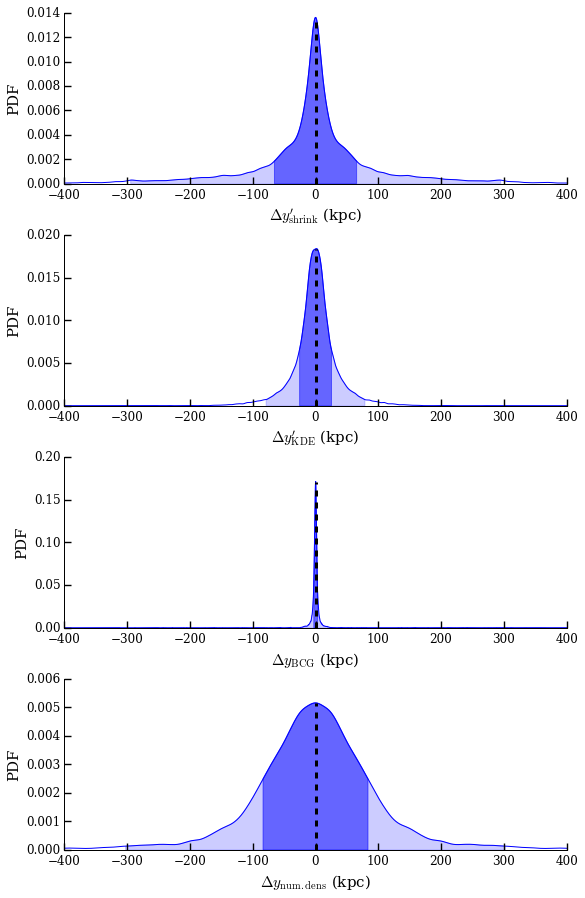
\includegraphics[width=0.65\linewidth]{fig5_symmetrical_1D_pdf.png}
	\caption{ 		
		The smoothed distribution of different offsets of 43 clusters with all 768
		projections. The smoothing bandwidth is determined by Scott's rule for 
		visualization.
		For estimates where several peaks of galaxy data are 
		possible, only the densest peak is matched to the DM peak for computing
		the offsets in this figure. 
		The dark blue area indicates the 68\% density interval
		while the light blue area shows the 95\% density interval. 
		The table summarizing the statistic of each distribution is available in
		table 
		\label{fig:offset_distributions}
	}
\end{center}
\end{figure*}

\begin{figure*}
	\begin{center}
	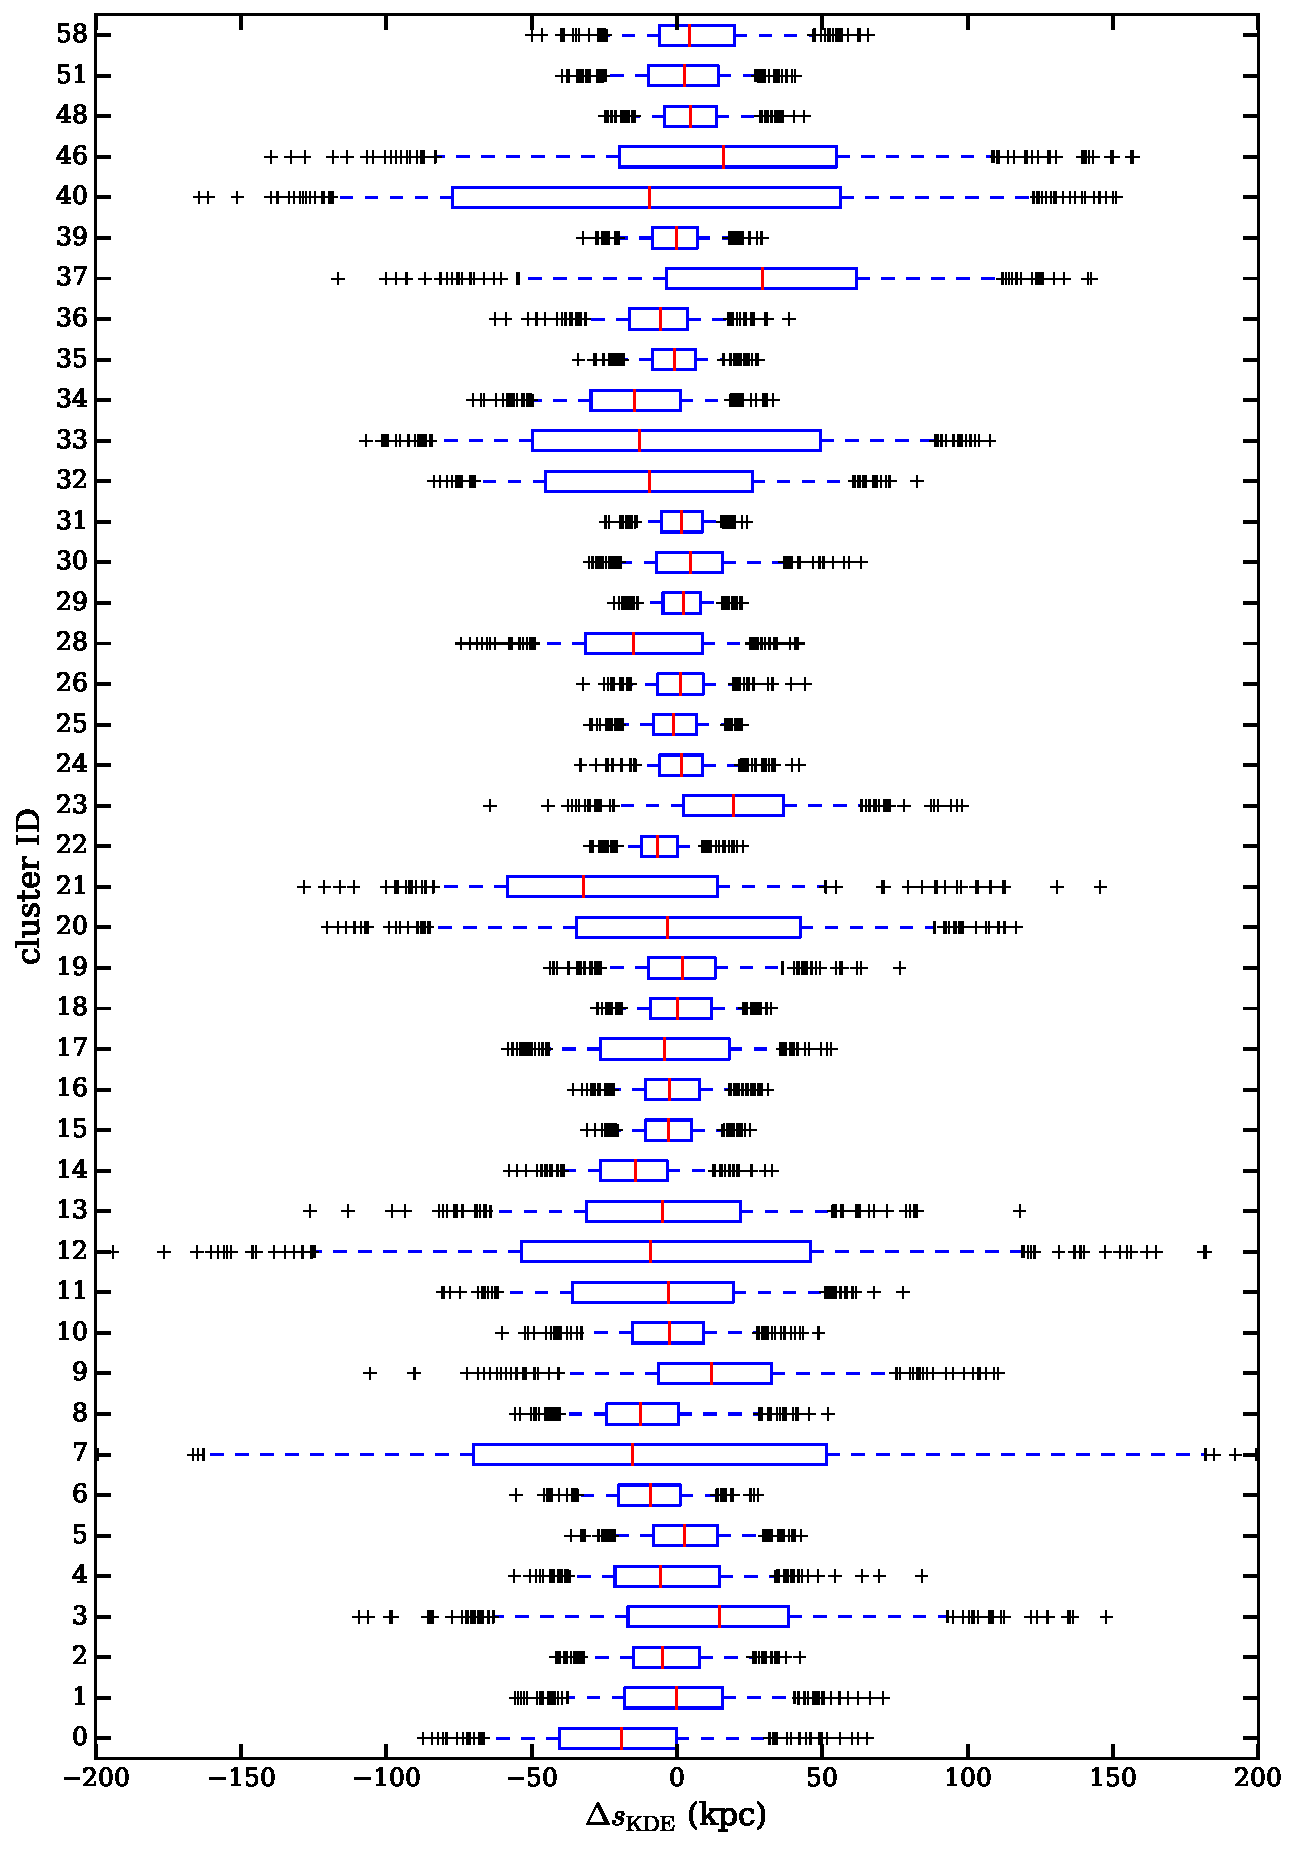
\includegraphics[width=0.85\linewidth]{fig7_projected_KDE_offset_distribution.pdf}
	\caption{A box plot showing the distribution of $\Delta y_{\rm KDE}$ for each cluster 
		based on 768 projections. The red line shows the median of the projections,
		the box encompasses the 25-th and 75-th percentile of the distribution while
		the whiskers mark the 5-th and the 95-th percentile. The other black crosses
		are data points with extreme values beyond the 5-th and 95-th percentile.
		The offsets were computed between the closest DM 
		peak to the brightest luminosity peak of each cluster. 		
		\label{fig:projected_KDE_offset_distribution}
	}
\end{center}
\end{figure*}

\subsection{Offset projection uncertainty of each cluster}
When we gather the offsets $\Delta s_{\rm KDE}'$ of the 
768 projections for each cluster,
we can find the offset uncertainty due to projection effects.
The distributed are illustrated in the box plot of Fig. 
\ref{fig:projected_KDE_offset_distribution}. The values of the biweight mid-
variance of $\Delta y_{\rm KDE}'$ for half of the clusters
are $< 23$ kpc. Of the ten clusters (ID = 3, 7, 12, 20, 21, 32, 33, 37, 40 and 46) 
that have mid-variance $ > 40$ kpc, all of them have the median of $\nu > 1.2$.
 
\subsection{Correlations between different variables and the offsets}

Here we investigate a list of physical quantities that have significant to little
correlation with the offsets. 
We use the Pearson product-moment correlation coefficient to quantify linear 
relationship between the pairs of variables. 
(aka Pearson's r,  hereafter $\rho$)
We describe the significance of the correlation 
based on the p-value reported by {\bf \texttt{Scipy}} of seeing the level of 
correlation by chance assuming the pair of 
quantities have no correlation. If the p-value is greater than 0.1, we call the
correlation as insignificant.
As a reference, the correlation of between the 
unrelaxedness criteria defined in section \ref{subsubsec:relaxedness}
for the 43 selected clusters is as high as 0.82. 

Each of the unrelaxedness have significant a positive correlation of $\sim 0.70$
with the maximum of $\Delta s_{\rm KDE}'$ of each cluster
(hereafter $\max(\Delta s_{\rm KDE}')$).
The offset $\max(\Delta s_{\rm KDE})'$ per cluster also show a high
correlation of 0.77 with the median $\nu$ per cluster (hereafter,
median($\nu$)). The FoF mass of each cluster shows only slight correlation of 0.28 with 
 median($\nu$).

There is weak correlation between the richness of the
clusters with $\max(\Delta s_{\rm KDE})$ ($\rho = 0.21$). This weak correlation 
may be due to 
the fact that the peak estimate is only affected strongly by a few bright galaxies near 
the peak. The richness is slightly more strongly correlated with the median of $\nu$ 
with $\rho = 0.33$. 

There is insignificant negative correlation ($\rho = -0.20$) between the different mass 
measured within a certain density threshold, such as $M_{200C}$, $M_{500C}$, 
and $\max(\Delta s_{\rm KDE})$. The quantities $M_{200C}$ and $M_{500C}$, which
are computed within a shell centered on the most bound particles, have
symmetry assumptions that may not capture the total mass well if there are substructures. 
The FoF mass, which
captures the total mass without any symmetry assumption, correlates positively
and weakly 
($\rho = 0.13$) with $\max(\Delta s_{\rm KDE})$. 



% We subset the data and visually inspected the samples with the largest 
% galaxy-DM offsets $\Delta s_{\rm KDE}$. We found that ...  
% 
% \subsubsection{Correlations between the offsets and properties of the 
% cluster / groups}
% [TODO] examine the relationship between
% \begin{itemize}
% \item 3D relaxedness
% \item mass 
% \item richness  
% \end{itemize}
 
 
 
\section{DISCUSSION}\label{sec:discussion}

\subsection{Other findings from the visual inspection of the simulated galaxy clusters}
We inspected both the luminosity maps and the
number density maps of the member galaxy populations.
With the same selection of bright galaxies of apparent $i$-band$ < 24.4$ at
$z=0.3$, the luminosity maps in general resemble the DM maps more closely than 
the number density maps.
A comparison of the projected 
DM map, the luminosity map and the number density map of 129 clusters 
can be found at \href{https://goo.gl/kZUWrg}{https://goo.gl/kZUWrg}, 
\href{https://goo.gl/R7VNi9}{https://goo.gl/R7VNi9} and
\href{https://goo.gl/lmQUPd}{https://goo.gl/lmQUPd} respectively. 
We encourage our readers to view the luminosity map to see how it is possible
to create scientifically accurate contours of the DM distribution if the member galaxy
data is of high completeness and purity. The KDE is not just a fancy way of
identifying possible BCG candidates close to the luminosity peaks.
(As
 the high resolution figures need to be downloaded, the 
corresponding Jupyter notebooks may take some time and several refresh of the
web page before they are rendered properly.)

In real observations, missing selection of member galaxies, or 
foreground objects can both affect the inference of the galaxy spatial 
distribution. The number density map can be less susceptible to bias from bright 
foreground objects. It is less clear about the effect of missing member galaxies 
for computing the luminosity map because there is a selection bias favoring 
bright member galaxies.

\subsection{Comparison to merging cluster observations}

The offset distributions in table \ref{tab:p_val_table}
represent an estimation of the spread of $\Delta s$ in a $\Lambda$CDM universe.
While the compilation of the offset distribution suffers 
from the small number of high mass clusters in the Illustris simulation, 
the distribution probes projection uncertainties comprehensively. 
Possible discrepancies that affect our comparison can arise
due to the high purity and completeness of the Illustris galaxy data.
Most observations of massive galaxy clusters with total mass of M$_\odot
\approx 10^{14}$ have richness $\lesssim 300$, while the most massive Illustris
cluster (M$_{\rm FoF} = 3.23 \times 10^{14} M_\odot$) has a richness of 483.
Furthermore, the Illustris clusters are less massive than the observed clusters
with huge offsets. The Illustris clusters may also provide sufficient samples
of possible spatial configurations of observed clusters.
Despite the possible differences, we try to do a
fair comparison to observation by matching the method of offset inference. 

Other complications can arise from how one choose to subset the offset estimate
based on the cluster properties.
The full sample in table \ref{tab:p_val_table} preserves the cluster mass-abundance
relationship, i.e. each cluster has the same number of projections in
the full sample. However, it also underestimates the offset spread because the
full sample includes $\sim 45\%$ of relatively relaxed projections 
that only have one primary luminosity component.  These clusters would
have been excluded for comparison with bimodal mergers. 
Subsetting with $1.2 < \nu < 2.2$ picks out
cluster projections that are in more similar dynamical states as the observed merging
cluster. 
However, some simulated clusters may have more projections included in this sample
than the other clusters. From inspection of the mass abundance relations in 
Fig. \ref{fig:mass_abundance_distribution}, we found that subsampling with $1.2 <
\nu <2.2$ includes a higher proportion of projections from massive clusters
($\sim 20\%$ more) than 
the full sample. This sampling should not introduce significant bias. 
The observed merging clusters are still more massive than the unrelaxed samples. 

We compile table \ref{tab:offset_results} with the corresponding lower bounds
for the p-values using
the $\Delta y$ distributions of the unrelaxed samples ($1.2 < \nu < 2.2$). 
The p-value lower bounds are reported base on the $\Delta y$ distribution 
from the same methods that the observed values were computed. 
The majority of the p-values from table \ref{tab:offset_results}, 13 out of 15, are
$ > 0.05$, only 2 p-values are below 0.05. 
This means the observations are mainly consistent with the null hypothesis: 
It is possible to see offset values as extreme as reported by observations
in a CDM universe. 
However, this does not mean that the CDM model is more probable than the SIDM model. 
The full physical implications of this result is rather involved so we defer
the discussion only for interested readers in section [TODO]. We continue to 
discuss the possible use of \ref{tab:p_val_table} and
the p-values in tables \ref{tab:offset_results}.

To avoid any report from this study directly quoting a p-value, we did not
combine the p-values from different observations. 
This is because the computation of p-value does not fully
takes the true uncertainties of the observations into account. 
Most of the quoted uncertainties from \ref{tab:offset_results} are only 
from the lensing estimate, but not the error estimates of the galaxy summary 
statistic. 
Any future studies that wish to claim significance or rejection based on
comparison to a simulation will 
need to carefully track down the contribution of uncertainties from each aspect
of the cluster analysis.  
It may be reasonable to inversely weight offsets by the 
reported bootstrapped uncertainty $|\Delta s_{\rm KDE}|$ for each cluster.

As warned by the American Statistical Association in a statement [TODO],
p-value can be misinterpreted easily, so
we must take caution in the procedure of computing and interpreting the p-values. 
For example, the high energy physics community deliberately set the detection
threshold to be 5 $\sigma$ to account for how systematic and bootstrapped 
uncertainties can be
underestimated or unaccounted for. 
If the reliability of each observation is 
approximately the same, averaging the p-values can be one way of combining the p-values 
but there is no consensus of the best practice of combining the
p-values. The rule used to combine the p-values 
needs to be carefully designed according to the goal of the experiment.
When one keeps on including more observations,  
there will be some observations with extreme p-values that greatly influences the
overall p-value. It is necessary to adjust for the sample size for such running
experiments.   
The particle physics community,
for example, discusses how to set stopping rules [TODO add reference]
to account for the sample size to determine what p-value level should indicate meaningful
discrepancies from the expectation of the null hypothesis {\it before}
analyzing the data. 
How to count the sample size, i.e. whether to count the offsets from the same
system as the same sample, is a subject up for debate.
Regardless, computing a combined p-value for all the listed observations alone does not help 
understand how to best constrain SIDM.
We instead focus on discussing possible ways to build on top of the results
of this study and improve the design of the 
analysis in section [TODO]. 

\subsubsection{Comparison of the offset results to studies of clusters and groups}
Our results showing offset distribution are highly relevant to two other types of
observational studies: 
The first type tries to map the DM distribution of galaxy clusters 
using lensing techniques. 
The second type focuses on finding the best way to stack galaxy groups for
inferring cosmological parameters from the galaxy cluster mass function.
In the following section, we will show that cosmological simulations generally show 
the BCGs has the tightest offsets from the DM peaks, which is consistent with
our finding.
Observational studies, however, in general do not find offset as tight as the 
simulations. We discuss some factors (other than SIDM) quoted in the literature that 
have shown to affect the observed offsets, including the lensing resolution and the
choice of summary statistic for the member galaxy population. In particular, 
in the comparison of the luminosity peak to other galaxy summary statistic,
the luminosity peak shows promise to give the second least amount of bias,
after the BCG. 
 
To establish the baseline of the tightest $\Delta s$, we first discuss and 
compare the $\Delta s_{\rm BCG}$ constraints.   
\cite{Cui2015}, using 184 galaxy clusters with M$ > 10^{14}$ M$_\odot$ in a
N-body and hydrodynamical cosmological simulation suite powered by GADGET-3, 
% simulation suite with two types baryonic feedback prescription models,
% including radiative cooling, start formation and supernovae feedback, but one with feedback from Active
% Galactic Nuclei (AGN) and one without, \cite{Cui2015} 
also identified the maximum smoothed particle hydrodynamic (SPH) density peak
to summarize 
the galaxy population in their cluster samples. \cite{Cui2015} found
most offsets between BCGs and the most gravitationally bound particle to be
mostly below 10 $h^{-1}$ kpc. They also reported some extreme outliers 
spanning up to several hundred $h^{-1}$ kpc due to the disturbed cluster morphology. Our 
tight 68-th percentile of 
$\Delta y_{\rm BCG}$ at $ \pm 3$ kpc gives some confidence that 
we have identified most of the BCGs correctly in the Illustris simulation.

The distributions of $\Delta s_{\rm BCG}$ derived from simulations, in general, 
are less spread out than those computed in most observational studies.
For example, \cite{Oguri2010} have analyzed 25 X-ray luminous 
massive galaxy clusters of the LoCuSS survey. 
Observations were performed with a large FOV ($\sim 3 h^{-1}$ Mpc) 
using the Subaru Suprime Camera. 
By fitting elliptical NFW models to the weak lensing data, \cite{Oguri2010}
showed a long tail
 distribution for $\Delta s_{\rm BCG}$, which they fit with two 2D Gaussians.
The first tighter 2D Gaussian had a standard deviation being 90
$h^{-1}$ kpc for describing the
offset for most clusters, the long tail spans around 1 Mpc was fit by a second 2D
Gaussian with a standard deviation of 420 $h^{-1}$ kpc. This second component
in the tail region contains $\sim$ 10\% of the clusters in the study and is
consistent with the number of extreme outliers that we have.   
Note that by subsetting to only consider relatively relaxed clusters, 
there is a tight maximum bound $\pm$19 kpc for $\Delta y_{\rm BCG}$ in our study. 

One major source of uncertainties for computing $\Delta s_{\rm BCG}$ is the
misidentification of BCG.
To see the effects of misidentifications of 
BCGs, some studies have made use of N-body hydrodynamical cosmological
simulations to compute the 2D distances between the BCG and 
the second most massive galaxies. \cite{Johnston2007b} and 
\cite{Hilbert2010} (using the Millenium simulation)  found 
the one sigma level offsets for misidentified BCGs at 380 $h^{-1}$ kpc, and 410 
$h^{-1}$ kpc respectively. This is consistent with the 95-th percentile of the
unrelaxed and the full sample of the BCG in our study and also the tail of the
$|\Delta s_{\rm BCG}|$ for \cite{Cui2015}. If one wishes to use BCG with high
confidence, it may be necessary to set stringent standard of the morphological
characteristics of the BCG for classification, e.g. a minimum half light radius.

Another source of uncertainty for $\Delta s_{\rm BCG}$ was from lensing. 
\cite{Dietrich2012} performed an analogous analysis of the work of \cite{Oguri2010} 
using the N-body Millenium Run (MR) simulation.
They showed that a combination of shape noise and modeling choices 
alone can lead to hundred-kpc-level offsets between the most bound particle 
(proxy of the BCG) and the lensing peak for cluster-sized DM halos 
(M $> 10^{14 }M_\odot$).  
\cite{Dietrich2012} ray-traced through the DM substructures in the MR simulation 
as mock lensing observation of 512 clusters.  
Without any smoothing and shape noise, \cite{Dietrich2012} showed 
90\% of the lensing peak and the 
most bound particle, which is a proxy for the BCG, agree to 2.0 $h^{-1}$ kpc. 
With shape noise,
even at the source galaxy density of space-based quality optical data of n = 80
arcmin$^{-1}$, fitting NFW halos and using the center as the DM gave a 
distribution of $|\Delta s_{\rm BCG}|$ those mode is at around 9 arcsecs (this is
approximately the 1 standard deviation estimate in 2D).
Lowering the source galaxy density to 30 arcmin$^{-1}$ increased the mode
to 22 arcsec with a 95-th percentile at 85 arcsec 
($\sim 90$ kpc and $\sim 400$ kpc at z = 0.3, comparable to \citealt{Oguri2010}). 
Smoothing, in the presence of shape noise,
resulted in an offset distribution with the mode at
15 arcsec ($\sim 60$ kpc at z = 0.3). 
The offsets do not simply depend on the smoothing bandwidth, 
but also the number density of the source galaxies that are lensed. 
While the uncertainty from smoothing the DM map is
relatively unimportant in the Illustris analysis due to the much higher resolution 
of the DM particles than the sparser source galaxies used for lensing, it
highlights why the bootstrapped uncertainties from the observed
DM peak need to be accounted for during the comparison between the
Illustris results and the observations.

It is noteworthy from the work of \cite{Dietrich2012} that 
smoothing alone can caused the peak offset to shift from several arcsecs to
around 1 arcmin.
Any other morphological features from the smoothed DM map will be subject 
to uncertainty of similar order of magnitude as the peak
estimate, but with lower signal. 
There is also a risk of seeing substructures that mimic the sought-after 
morphological patterns. After all, other cosmological experiments 
that have shown
that it is possible to detect patterns once scientists look hard enough, 
such as the initials of Stephen
Hawking in the seventh-year Wilkinson Microwave Anisotropy Probe (WMAP) 
Cosmic Microwave Background data \citep{Bennett2011}.

Now we turn to exploring complementary methods for summarizing
the galaxy population of a cluster, and show that  the luminosity peak 
is the second best choice than the BCG for summarizing the galaxy statistic.
A unique BCG does not always exist for a cluster (or the subcluster).   
Bright galaxies in the dense region of the cluster are the possible progenitors 
of the BCG and therefore a reasonable choice when there is no unique BCG. 
\cite{George2012a}, for example, examined 129 X-ray selected non-merging galaxy 
groups in the COSMOS field.
They found that around 20\% to 30\% of groups have non-negligible discrepancies
between different galaxy centroids. 
By stacking on a bright galaxy near the X-ray centroid, they found  
the resulting lensing strength is higher than the stacked lensing signal based
on other galaxy centroids, including the BCG. 
For groups with clear BCG candidate, \cite{George2012a} gave the range of
offset between the BCG and the assumed halo center as $\lesssim 75$ kpc. 
The KDE peaks from the luminosity maps of the Illustris samples show a much 
tighter offset to the 
lensing center than any other centroids that \cite{George2012a} investigated. 
The weighted or unweighted centroid measurement from \cite{George2012a} has a 
$|\Delta s|$ with standard deviation at 50 - 150 kpc from the
lensing center with long tails (of around several hundred kpc). 
In comparison, the median (26 kpc), mean (37 kpc), standard deviation (35 kpc) 
and 75-th percentile (49 kpc) of 
$|\Delta s_{\rm KDE}|$ from all the Illustris samples are below 50 kpc. 

We attribute the small amount of population bias of $\Delta s_{\rm KDE}$ in our
analysis due 
to cross validation, a well-tested procedure accepted by all the top journals 
from the statistics and the machine learning communities. 
Not only does the algorithm help
determine the eigenvalues, but also the optimal eigenvector direction of 
the bandwidth matrix. 
Most literature do not discuss how the bandwidth of 
the kernel for the smoothed maps are determined.  
It is unclear if such results will enjoy the same accuracy level as what
we demonstrated. 
If scientists hand tune the smoothing bandwidth, it is hard to
avoid setting the bandwidth to fit the preconception of how the density
contours of the cluster 
should look like, and inadvertently biasing $\Delta s$.

% [This study is too weird to be included - the FOV is unusually small]
% The feasibility of using luminosity peak as a complementary method to represent
% the galaxy population has also been verified in observations.
% Using 10 000 Sloan Digital Sky Survey (SDSS) galaxy groups and clusters 
% in the Gaussian Mixture Brightest Cluster Galaxy (GMBCG) catalog \citep{Hao2009},
% \cite{Zitrin2012} were able to use the smoothed luminosity maps of the red-sequence 
% galaxies to locate the BCG, which the authors assumed to be the proxy of the DM peak. 
% The richness of the groups range from tens of members to around 160 members. 
% After optimizing the different degrees of smoothing polynomials and 
% assuming a power-law spatial distribution of galaxies, \cite{Zitrin2012} found
% a 24-th degree spline interpolation to best fit the galaxy data within a small
% assumed FOV of
% 120 arcsec$^{2}$  for a luminosity peak. (This FOV translates to 
% $\sim$ 110 $h^{-1}$ kpc$^2$ for the redshift range in the
% paper \citealt{Zitrin2012}). The densest luminosity peak from the spline interpolation had 
% a very close agreement with the identified BCG those mode is $\sim$ 4.2
% $h^{-1}$ kpc after removing 12\% of outliners those offsets are about as wide
% as the FOV. 

% There are also possible differences in the accuracy of our peak
% estimation method and other studies. 
% The population mid-variance of $\Delta y_{\rm KDE}$, which quantifies the
% population bias from the DM peak estimation, is 23 kpc (the 68-th percentile is
% $\pm$ 25 kpc).

[TODO revise this paragraph]
% Finally, we try to conclude this subsection by discussing how the offset 
% information of different summary statistic of a cluster can help center the cluster for
% stacked lensing analysis. 
% The equation for modeling the density for stacked clusters usually 
% involve a density term for the BCG,
% one halo term centered on the BCG, some miscentering correction, and a nearby
% halo term \citep{Johnston2007b}. 
% When the galaxy summary statistics disagree (offset $> 50$ kpc),  
% the BCG (and luminosity peak) often land on top of one of the dense subcomponents
% of a generally asymmetrical spatial distribution.
% The weighted centroids,  
% which are the proxies for the center of mass for these disturbed clusters,
% on the other hand, often land in between dense substructures.
% For such an asymmetrical cluster, 
% there is no point location that will simultaneously satisfy the
% requirements of 1) maximizing the density, and 2) preserving symmetry.
% If a high precision is required, one can do it at the sacrifice of a smaller sample size. 
% One can only stack clusters those galaxy summary statistics, e.g.
% the centroid and BCG (or the luminosity peak), have high degree of agreement.
% To take care of the complex morphology for clusters with multiple components,
% a more sophisticated stacking model is needed.
 
  
\subsection{Comparison to staged simulations with SIDM}
\label{subsec:SIDM_sim}
Staged simulation are controlled experiments for probing the contribution
of SIDM to offsets in mergers of cluster components. 
The non deterministic nature of particle interactions means that it is not easy
to predict the offsets analytically.
There is no consensus of what type of clusters might best show the effects of SIDM.
This is because the effects are dependent on the model of SIDM.
Currently, the studies of SIDM have been restricted to those with isotropic
scattering and velocity-independent cross sections.   
The two main classes of SIDM that are studied include those with 
frequent, short-range interactions that can be broadly be modeled by an
effective drag force, and those with rare, longer range interactions those
effects are not well described by a drag-force approximation \citep{Kahlhoefer14}. 
In addition having a dependence on the merger configurations, the offset due to
SIDM also has a time-dependence.    

At SIDM cross section level favored by current literature $\sigma_{\rm SIDM}
\lesssim 1 \centi\meter ~\gram^{-1}$, a list of SIDM simulation studies (Kim \&
Peter 2016, \citealt{Robertson2016}, \citealt{Kahlhoefer14}, \citealt{Randall2008d})
have reported that, during the offset is observable, 
offset generally scales linearly with $\sigma_{\rm SIDM}$. 
However, most of the upper limit of the offsets due to SIDM to are of the order of magnitude 
of 50 kpc. 
For simulations of major mergers of two subclusters, it takes time for the self-interaction of DM
to manifest and lag behind the galaxies. Kim \& Peter (2016), for example, showed that
this lag starts to be observable approximately after the subclusters reached apocenter. 
While the offset may persist when the subclusters are returning for a
second collision, the magnitude of the offset can fluctuate over this period.
In general, the offset is affected by the phase of major mergers that cannot be
accurately estimated.

This small level of offset due to SIDM rules out the use of most summary 
method of galaxy statistics for computing SIDM constraints. 
The uncertainties overwhelm the signal. 
A offset level of 50 kpc is within the one-sigma level of $\Delta s_{\rm num.
dens}$, $\Delta s_{\rm shrink}$, and $\Delta s_{\rm centroid}$, the two-sigma
level of the $\Delta s_{\rm KDE}$. Despite $\Delta s_{\rm BCG}$. 
 has tight distribution for relaxed clusters, misidentification of the BCG 
may increase the tail of the distribution to render it unsuitable to be used 
for secure constraints. And to sample the tight distribution at higher
resolution than provided here, a simulation at galactic scales with realistic
baryonic feedback will be needed.   

\section{The role of CDM cosmological simulations for 
statistically inferring SIDM from a population of galaxy clusters} 
  
So far the analysis has focused on comparing the offset uncertainties 
from the inference methods and the SIDM offset signal, but we must emphasize 
that the high level of uncertainty from CDM simulation matching the observed level is
insufficient to rule out small SIDM cross section.  
We have not shown if realistic mock observations of cosmological simulations of SIDM 
with small cross section would match observations in better or worse ways. It is
also possible that the SIDM results would be largely indistinguishable from our results. 
This is because the uncertainties from the offset inference method is not
guaranteed to bias the offset level high. Also having an small SIDM cross section
only produces offset under restricted set of merger configurations. 

Assume we have chosen a certain offset estimation method and to study $n$ clusters
of a certain mass range and dynamical states (i.e. merger with $ 1.2 < \nu < 2.2$),
the distribution of population observed offset signal 
has two main contributions that we assume to be
independent:
\begin{equation}
	\Delta s_{\rm obs} =  \Delta s_{\rm SIDM} + \Delta s_{\rm noise} 
\end{equation}

From our analysis, we showed that for most of the observation methods, 
$\Delta s_{\rm noise}$ has an approximately zero mean and a certain covariance
matrix. We need to evaluate a few things before deciding whether the contribution
from $\Delta s_{\rm SIDM}$ with a certain cross-section will create a second
peak excess for $\Delta s_{\rm obs}$ away from zero. 
The distribution of $\Delta s_{\rm SIDM}$ depends heavily on the
fraction of merger configurations that can give non-zero offset signal of SIDM
given a cross section, 
the SIDM offset distribution of such mergers and 
the chance of picking such merger configurations to observe over the total
observed population. 
As we know that the mean offset signal of SIDM, within the cross section range favored by
current literature,
is close to the peak of the $\Delta
s_{\rm noise}$ distribution, 
if $\Delta s_{\rm SIDM}$ from the chosen mergers have high enough variance, 
studying more mergers will not result in an excess of population offset signal
of SIDM at any characteristic length scale, when compared to $\Delta s_{\rm
noise}$. 
Although, even in the optimistic case that one figures out how to pick mergers to create
a population offset signal excess at a certain length scale, 
there are practical limits on how well one can find them in observations. 

 
% Strong lensing but that brings the signal done 
% 
% In most available theories and simulations for observing offsets due to SIDM, 
% depend on a combination of the concentration of the merger components,  
% the impact parameter, the merger velocity, and the time relative to the merger. 
% 
% 
% 
% 
% 
%  
% 
% 
% The measurement cluster components is prepared such that the measurement 
% uncertainties are mostly negligible and all the offset signals are contributed
% by interactions from SIDM.
% This assumption is confirmed by test runs where $\sigma_{\rm SIDM} = 0 \centi\meter^2
% \gram^{-1}$ consistently report offsets $< 5$ kpc (\citealt{Randall2008d}, 
% \citealt{Kahlhoefer14}, Kim \& Peter 2016). 
% While there are many analytical theories of the observables due to SIDM 
% that may provide order-of-magnitude estimations, 
% they have not shown that the DM in the observed systems, 
% under the inferred $\sigma_{\rm SIDM}$ level,
% can produce the level of signal  
% (\citealt{Massey2011}, 
% \citealt{Harvey2015}) are not validated in SIDM simulation. 
% 
% 
% 
% different class of SIDM models that 
% 
% dynamical 
% There 
% In fact, the SIDM simulation suites have provided different insights to
% 
% offset may have a dependence on the time-since-pericenter of the merger
% cannot distinguish between offset  
% 
% 2 types of SIDM to test for 
% 
% 
% Therefore, we focus on comparing the offset levels of the Illustris
% clusters, the listed observations in \ref{tab:offset_distributions} 
% to the quantified offsets in staged SIDM simulations. 
% 
% The quoted staged SIDM simulations here (Kim \& Peter 2016, 
% \citealt{Robertson2016}, \citealt{Kahlhoefer14}, 
% \citealt{Randall2008d}) represent some of the maximal 
% offset signal that can be detected due to SIDM. 
% This is because of the denser assumed halo
% core ($10^{14} M_\odot < M < 10^{15} M_\odot$) for the high mass binary 
% mergers. In the mentioned
% staged simulations, most of the mechanisms
% through which SIDM produces an offset in a merger have strengths proportional
% to the mass density $\rho_{\rm mass}$ of the infalling halos.  
% Subclusters infalling into the main cluster, not only may not produce offset of 
% an observable magnitude, it is harder to determine their peaks with high enough 
% accuracies due to the lack of strong lensing information. As discussed in the 
% previous section, 
% the peak determination of weak lensing peak of massive cluster also has low
% signal to noise ($\sim$ 1:1). 
% 
% In fact, \cite{Kahlhoefer14} has argued that only SIDM with frequent
% interaction rates can be represented by an effective drag force, and this is assumed
% by the aforementioned analytical theories.
% 
% offset is highly dependent on merger parameters (Kim \& Peter 2015) 
% 
% 
%  If there is a spectroscopically confirmed BCG member of the 
% cluster and strong lensing information,
% 
% How do you propagate the uncertainty to Morphological features? 
% Quantify morphological features, the presence / absence of morphological
% features is subjective 
% 
% features can be measured but cannot be untangled from the statistical uncertainties.
% 
% 
% Types of SIDM interaction that were not considered before.
% 
% Central limit theorem states that the means of iterates of random variable
% drawn from a known distribution of finite variance 
% 
% 
% The bootstrapped distribution(s) of offset per clusters do not necessarily 
% resemble one another. 
% This means the offsets are not guaranteed to enjoy the benefits from the 
% central-limit-theorem 
% because they are not drawn from an identical distribution. 
% 
% 
% Offset is a complicated function of the time-since-pericenter of major mergers,
% impact parameter, 
% 
% 
% Zoomed simulation from Rocha et al.
% 
% 
% % Statistical uncertainties overwhelm the signal of SIDM.
% N-body interaction 
% Can an analytical theory predict the effects of SIDM without simulation. 
% show the analytical argument have order of magnitude accuracies 
% have not shown that the $|\Delta s|$ signal 
% is above detection limit. 
% 
% Robertson2016 said that the stripped gas can introduce asymmetry in the
% cluster spatial distributions  
% 
% \cite{Harvey2015}
% Have not examined how well their theory works in SIDM simulations
% 
% ignored the dependence of mass, surface area and the drag coefficient 
% of the galaxies and the DM 
% 
% 
% 
% The projection uncertainty, the measurement uncertainty shown both by
% individual observations and in this study   
% on par with the SIDM signal.
% the bootstrapped uncertainties are several times the possible signal level,
% which may be observed in very specific time-window and configurations 
% 
% uncertainty can account for at least half of the offset signal
% 
% \cite{Kahlhoefer14}
% \cite{Randall2008d} can be thought of a controlled experiment where 
% % only the effects of SIDM is in place.
% 
% ambiguous proposal of observables 
% 
% 
% 
% % % This is because a large number of tracer galaxies were painted on as 
% % collisionless particles, using identical distributions between the galaxies 
% % and the DM particles at the beginning of each run. 
% 
% % In this work, we test purely for the offset due to statistical noise and
% % missing variables such as projection and impact parameter 
% % there is not enough evidence there is not enough evidence there is not enough evidence 
% % 
%  
% 
% 
% 
% % [TODO] cite Stacey
%  
% % It is not clear about the ability of $\Delta s_{\rm SIDM}$ for differentiating 
% % between different $\sigma_{\rm SIDM}$ models. 
% % 
% % It is unclear that $\Delta s$ is a sensitive observable to signatures of
% % $SIDM$.
%  
% % At $\sigma_{\rm SIDM} \approx 1.25 $cm$^2$ / g, 
% % \citealt{Randall2008d}, \citealt{Robertson2016} only found an offset of $50
% % kpc$, this is completely within the population uncertainties of offsets, 
% % while the projection uncertainty of a cluster can be as large as  
% % [TODO]$ $ kpc.
% % 
% % 
% % Bullet cluster  
% % \subsubsection{Estimation of the SIDM cross section from the Illustris offsets}
% % Since the Illustris simulation assumes CDM, it is interesting to see if we can
% % infer any non-zero $\sigma_{\rm SIDM}$ from the offset estimates based on
% % different methods.  
% 
% 
% There are also questions that theorists and analysts formulating the
% statistical models need to answer:
% Bootstrapped uncertainties of the source galaxies in the lensing map 
% Why are uncertainties due to smoothing and substructures, e.g. imperfect
% fitting of asymmetrical data by the assumed symmetrical halo profiles, 
% get translated into increased probability of having self-interaction
% dark matter? If  
% 
%  
%  
% 
%  
% % \subsection{How to use $\Delta s$ to constrain $\sigma_{\rm SIDM}$}
% % 
% Statistical aspects that one should take into account when constructing such a
% test include: 
% \begin{itemize}
% \item whether the population PDF of offsets have converged  
% \end{itemize}
%  
% Characterizing the state of the cluster is not trivial.
% 
% high dimensional space suffers from the curse of dimensionality 
% 
% 
% % % 
% % 
% % When there are real observations that lie sufficiently far away from the 95\% 
% % confidence region of the population distribution of the Illustris offsets, 
% % it is less likely that the null hypothesis that $\sigma_{\rm SIDM}$ is true.
% 
% 
% propagation of error 
% non-deterministic 
% monte Carlo simulation 
% do not contain the right level of physics 
% what are the needed physics?
% predict strength of the SIDM drag force due to macroscopic properties 
% dynamical friction, correct clustering scaling of substructures   
% 
% as there is no deterministic model predicting the effects of SIDM given the 
% properties of a galaxy cluster, it is hard to propagate and account for 
% observational uncertainties. 
% 
% causes of offsets that are not SIDM 
% 
% imperfect characterization of substructures 
% contours - avoid any assertions of symmetry requirements  
% smoothing 
% 
% it is interesting to think of the implications of the large statistical 
% uncertainties of $\Delta s$ for the inference of SIDM.
% 
% if SIDM gives a fixed offset signal for all clusters, then using more clusters
% will increase the signal strength and lead to an excess for a certain offset. 
% however, most SIDM particle interactions depend on the surface mass
% density and the net velocity of motion among subclusters, even though the definition 
% 
% directional lag - one such statistical test is called the Rayleigh z test  
% however, dynamical friction, ram pressure slingshot have to test for both the
% cDM and SIDM scenario with realistic distributions and numbers of member galaxies.  
% if the snapshot duration is short enough
%  one may track subhalos across snapshots to know confirm the
% direction of motion  Subject of investigation of another paper 
% 
% 
% 
% - have to be account for the uncertainty of the actual merger
% axis and the impact parameter  
% 
% 
% with the large uncertainties from observation studies as shown by the offset
% uncertainties in table \ref{tab:offset_distributions} and from fig. 
% 
% there are more statistical aspects that one need to consider before a rigorous
% comparison can be 
% 
% 
% the main implications of our results for inferring $\sigma_{\rm SIDM}$ from the
% offset are the following.
% 
% there is no deterministic one-to-one mapping between $\Delta s$ and 
% $\sigma_{\rm SIDM}$.  
% this result does not mean that $\sigma_{\rm SIDM}$ is always overestimated from
% past literature. 
% on the contrary, it means that individual SIDM offset estimate may either
% experience a random increase or decrease due to the statistical noise of 
%  the data and different offset inference methods have different sensitivity to 
%  the noise.
% if the offset signal from SIDM is small enough, the offset distribution may be
% degenerate between different $\sigma_{\rm SIDM}$ values.
% 
% 
% plagued by expensive observations and small number of cluster samples.
% very unlikely to find an analogous cluster to observations in a cosmological simulation 
% due to both the curse of dimensionality and missing variables such as
% line-of-sight information.
% multiple comparison 
% 
% not a statistically sound way of rejecting $\sigma_{\rm SIDM} = 0$
% warn against p-value 'hacking` using this Illustris data
% 
% 
% sound statistical analyses to claim discovery  
% 
% need expensive cosmological simulations with SIDM to gather sufficient statistics 
% 
% 
% since SIDM is not the only source of contribution to the galaxy-DM offset 
% in galaxy clusters,
% any method for small number of clusters do not account for the intrinsic 
% scatter will have unknown bias the estimate of $\sigma_{\rm SIDM}$. 
% this is because the statistcal scatter of $\Delta s$ may or may 
% not align with the SIDM offset contribution. 
% 
% need to sample enough galaxy clusters with the same selection criteria, 
% both from simulations and from observations.
% 
% asymmetry of DM map may not be statistically strong signal.
% failure of locating the peak with the strongest signal to noise 
% 
% 
% different choice of the size of smoothing kernel and projection effects can the
% other features in the spatial map.
% lead to spurious features such as tails in the convergence map.
% 
% in simulation 
% show low statistical noise floor so that 
% the selected observable of SIDM can discriminate between CDM and SIDM.   
% 
% hard to formulate a multivariate probability distribution to account for all
% the uncertainties from 
% time-since-collision, impact parameter, concentration of clusters before infall
% 
% how to characterize subclusters - 
% use different statistical methods for clustering the DM and galaxy 
% population. 
% using NFW halos for DM halos and using
% gaussian mixture model for galaxy clustering  
% not physical
% 
% 
% verify if cosmological simulations with a reasonable $\sigma_{\rm SIDM}$ value 
% have observable differences from the CDM simulations. 
% likelihood ratio: Bayes factor 
% 
% quantitative constraints carefully consider the contribution of each component
% 
% with the complications with analyzing galaxy clusters, 
% it is not clear that finding SIDM with galaxy cluster is a tractable problem. 
% 
% 
% 
% 
% 
% 
% modeling a galaxy cluster is a high dimensional problem with missing
% variables such as line-of-sight information and merging history which can all 
% lead to large uncertainties.
% 
% it is hard to define an analog for observed galaxy clusters due to missing
% information such as projection, merger history which may not be described well
% by parametric representation.
% 
% given the uncertainties purely due to offset estimation methods and 
% intrinsic scatter of $\Delta s$, any estimates of $\sigma_{\rm SIDM}$ without
% account for these uncertainties will overestimate. 
% 
% 
%  
%  
% 
% 
% no analytical form of how the effects of SIDM directly map as observables  
%  
% model fitting that takes  observational uncertainty into account. 
% 
% show unambiguous signal of SIDM that is detectable despite the noise 
% 
% occum's Razor, at least consider simple source of contributions to observed signal 
% before resorting to more exotic physics.
% 
% machine learning methods to paint galaxies to DM halos 
% http://arxiv.org/abs/1510.07659
% 
% 
\section{Future research direction}
the data in the Illustris simulation has proven to be an excellent source of
understanding observational uncertainties.
further work can be done to make mock observations more realistic, including:
\begin{itemize}
		\item adding foreground structures 
		\item adding more realistic peak detection threshold from the KDE luminosity map based on
			the flux per area at the peak location and compare that to observational
			limitations
		\item examining the effects of incompleteness removing some member galaxies randomly 
		\item computing the velocity dispersion of the galaxies along different
			line-of-sight to see how the velocity dispersion correlates the different
			measures of unrelaxedness
		\item testing for identifying member galaxies using the red sequence
		\item zoomed-in simulations of clusters with SIDM physics 	
	\end{itemize}


\section{SUMMARY}
We have shown that mock observations from simulations are important when there are no
theory mapping observables to $\sigma_{\rm SIDM}$. 
Kim \& Peter
2016 have shown that the SIDM offsets depend on the time of the merger, 
impact parameters, collisional velocity and mass concentration. 
There is yet to be an analytical model that includes all these merger parameters.
We cannot propagate observational uncertainty analytically when we compare
between theories and have to rely on simulations. 
we showed that 
\begin{itemize}
		\item it is possible to  
			see $\Delta s$ as extreme as those in observed merging galaxy clusters assuming that
			$\Lambda$CDM is the true underlying physical model  \\

		\item the contribution of statistical uncertainty to the galaxy-DM offsets 
			for $\Lambda$CDM clusters is not negligible when compared to the reported
			levels of offset from staged simulations ($\sim 50$ kpc). Any
			observational study that uses 
			galaxy-DM offsets to
			constrain $\sigma_{\rm SIDM}$ has to account for this contribution
			or else $\sigma_{\rm SIDM}$ will be biased. \\

		\item while the location estimates of the 2D spatial distribution of offsets and the
			1D spatial distributions of the offsets ($\Delta y$) in the Illustris
			simulation are approximately zero.
			The root-mean-square of the magnitude of the
			offsets is $\sim 30$ kpc from the Illustris sample. 
			If one uses the magnitude of the offset to constrain
			$\sigma_{\rm SIDM}$, $\sigma_{\rm SIDM} = 0$ 
			does not map to zero magnitude of offset.  
			The converse may also not be true but needs to be verify by a
			cosmological simulation with realistic galaxy distribution and SIDM. 
			\\

		\item with high completeness and purity of member galaxy data, the
			luminosity map resembles the DM spatial distribution more closely than 
			the number density map of member galaxies. \\ 

		\item the locations of the most gravitationally bound particle are consistent 
			with the BCG for systems with little substructures.  \\

		\item the BCG has the smallest offset to the dominant DM peak; and  
			the KDE peak of the luminosity map gives the second tightest 
			offsets from the DM peak. \\

		\item there are offset observations in the Illustris simulation that are as
			extreme as the offset observed in more massive merging galaxy clusters. 
			
		\item Lensing analysis that stack clusters based on the center of mass 
			will see miscentering due to 
			non-symmetrical and / or clumpy spatial distributions. 



		% \item the resolution of the DM distribution can affect
		% 	individual estimates $\Delta s$ but do not show significant bias for
		% 	the population estimate. However, the lower the resolution, the higher
		% 	the variance of the population estimate.  

\end{itemize}

furthermore, we have provided a set of python functions for making accurate 
contour levels for spatial maps and inferring density peaks at 
\href{https://goo.gl/MNrSQV}{https://goo.gl/MNrSQV}.
% 
% 
% 
% While this paper does not provide a solution to the complete statistical model
% for galaxy clusters, it points out some of the aspects that good models should
% incorporate, especially when the utility of studying the cluster is to
% constrain $\sigma_{\rm SIDM}$.
% 
% Aspects that should be handle with care include:
% \begin{itemize}
% 		\item the mass profile, especially when the cluster is multimodal 
% 		\item the evaluation of galaxy membership and the corresponding luminosity
% 			peak(s)
% \end{itemize}
% 
% 
% 


\section{ACKNOWLEDGEMENTS}
% Our software setup is available through a Docker image on DockerHub while the
% The main code are version controlled via Git and GitHub. 
kN would like to thank Professor Thomas Lee for the helpful discussion of 
the construction of the p-value hypothesis test. 

part of the work before the conception of this paper was discussed during 
the AstroHack week 2014. 
part of this work was performed under HST grant (TODO ask Dave for grant
number). 
% 
% 
% 
% % alternative ways of characterizing differences between DM and galaxy
% % distributions.
% 
% % \section{The Physical properties of a galaxy cluster}
% % State variables are missing.
% % A galaxy cluster is not a closed system. 
% 
% % correct for multiple comparisons
% % High number of latent variables 
% % have to rule out the possibility that observables of SIDM being affected by
% % the merger history of the cluster. 
% 
% 



\bibliographystyle{mnras}
\bibliography{galaxyDMoffset,Rpackage}
\appendix
\section{Algorithm of the Shrinking aperture estimates}
\label{app:shrink_apert}
\begin{algorithm}
	\caption{Shrinking aperture algorithm with luminosity weights}
	\KwData{subhalo that satisfy cuts as a galaxy}
	 \hrulefill \\

	 initial aperture centroid = weighted mean galaxy location in each spatial dimension\\
 	distance array = euclidean distances between initial aperture center and each galaxy
	location \\
 	aperture radius = 90th percentile of the weighted distance array\\ 
	\While{ (newCenterDist - oldCenterDist) / oldCenterDist $\geq$ 2e-2}{
 		new data array = old data array within aperture\\
 		newCenter = weighted mean value of new data along each spatial dimension 
	}   \hrulefill
\end{algorithm}

\section{Table of results}
\label{app:table_of_results}
\begin{landscape}
\begin{table}
	\begin{center}
	\caption{Properties of the clusters used in the analysis. Richness is
	computed based on $i-$band $< 24.4$ assuming $z=0.3$.\label{tab:cluster_prop}}
	\begin{tabular}{rrrrrrr}
\toprule
ID & richness & M$_{\rm 200C} (10^{14} M_\odot)$ & M$_{\rm 500C} (10^{14} M_\odot)$ & M$_{\rm FoF} (10^{14} M_\odot)$  & relaxedness$_0$ & relaxedness$_1$ \\
\midrule
 0 &      483 &                            16.35 &                            10.85 &                            32.29 &              29 &              33 \\
 1 &      338 &                            15.69 &                             6.16 &                            26.78 &              20 &              16 \\
 2 &      158 &                            15.33 &                             8.71 &                            21.20 &              17 &               3 \\
 3 &      134 &                             8.24 &                             5.63 &                            20.30 &              37 &              59 \\
 4 &      164 &                            11.93 &                             6.58 &                            15.42 &              21 &               4 \\
 5 &      115 &                             9.00 &                             5.65 &                            14.45 &              20 &              27 \\
 6 &       90 &                             9.58 &                             5.98 &                            14.01 &              18 &               7 \\
 7 &       92 &                             3.09 &                             1.74 &                            14.14 &              54 &             280 \\
 8 &      113 &                             8.25 &                             5.41 &                            13.36 &              24 &              26 \\
 9 &       97 &                             7.85 &                             4.98 &                            12.91 &              23 &              12 \\
10 &       83 &                             7.29 &                             5.33 &                            11.51 &              19 &               8 \\
11 &       86 &                             5.71 &                             3.32 &                             9.48 &              20 &               9 \\
12 &      267 &                             2.02 &                             0.87 &                             8.72 &              64 &             142 \\
13 &       84 &                             2.19 &                             1.43 &                             7.94 &              63 &             143 \\
14 &       89 &                             4.47 &                             2.88 &                             6.69 &              15 &               8 \\
15 &       70 &                             5.12 &                             3.50 &                             6.77 &              11 &               3 \\
16 &       68 &                             3.99 &                             2.30 &                             6.08 &              19 &               4 \\
17 &       66 &                             4.17 &                             1.84 &                             6.02 &              21 &               8 \\
18 &       79 &                             4.48 &                             3.15 &                             5.87 &              15 &               8 \\
19 &       61 &                             2.60 &                             1.85 &                             5.68 &              30 &              68 \\
20 &       69 &                             1.51 &                             1.08 &                             5.04 &              60 &             122 \\
21 &       62 &                             2.57 &                             1.23 &                             5.29 &              23 &               8 \\
22 &      343 &                             4.17 &                             3.05 &                             4.88 &              14 &               7 \\
23 &       59 &                             2.49 &                             1.72 &                             4.65 &              30 &              25 \\
24 &       57 &                             3.28 &                             2.62 &                             4.43 &              14 &              14 \\
25 &       56 &                             2.29 &                             1.50 &                             4.33 &              23 &              25 \\
26 &       69 &                             2.59 &                             1.81 &                             4.54 &              28 &              40 \\
28 &       63 &                             2.96 &                             1.64 &                             4.06 &              22 &              12 \\
29 &       69 &                             2.98 &                             2.05 &                             4.23 &              16 &              14 \\
30 &       72 &                             1.75 &                             1.36 &                             3.96 &              42 &              78 \\
31 &       63 &                             2.85 &                             2.12 &                             3.96 &              14 &              15 \\
32 &       55 &                             1.84 &                             1.29 &                             3.80 &              35 &              23 \\
33 &      213 &                             1.90 &                             1.03 &                             3.84 &              49 &              54 \\
34 &       54 &                             2.05 &                             1.41 &                             3.89 &              23 &              20 \\
35 &       52 &                             2.93 &                             2.17 &                             4.06 &              12 &               3 \\
36 &       53 &                             2.42 &                             1.62 &                             3.58 &              21 &              22 \\
37 &      212 &                             2.11 &                             1.55 &                             3.63 &              25 &              23 \\
39 &       56 &                             2.74 &                             1.79 &                             3.58 &              11 &               3 \\
40 &       58 &                             1.84 &                             0.99 &                             3.33 &              44 &              69 \\
46 &      225 &                             0.85 &                             0.58 &                             2.97 &              57 &              73 \\
48 &      230 &                             1.17 &                             0.85 &                             3.01 &              40 &             104 \\
51 &      148 &                             1.88 &                             1.34 &                             2.93 &              12 &               5 \\
58 &      187 &                             1.42 &                             0.88 &                             2.32 &              29 &              10 \\
\bottomrule
\end{tabular}

\end{center}
\end{table}
\end{landscape}

\begin{figure*}
	\begin{center}
	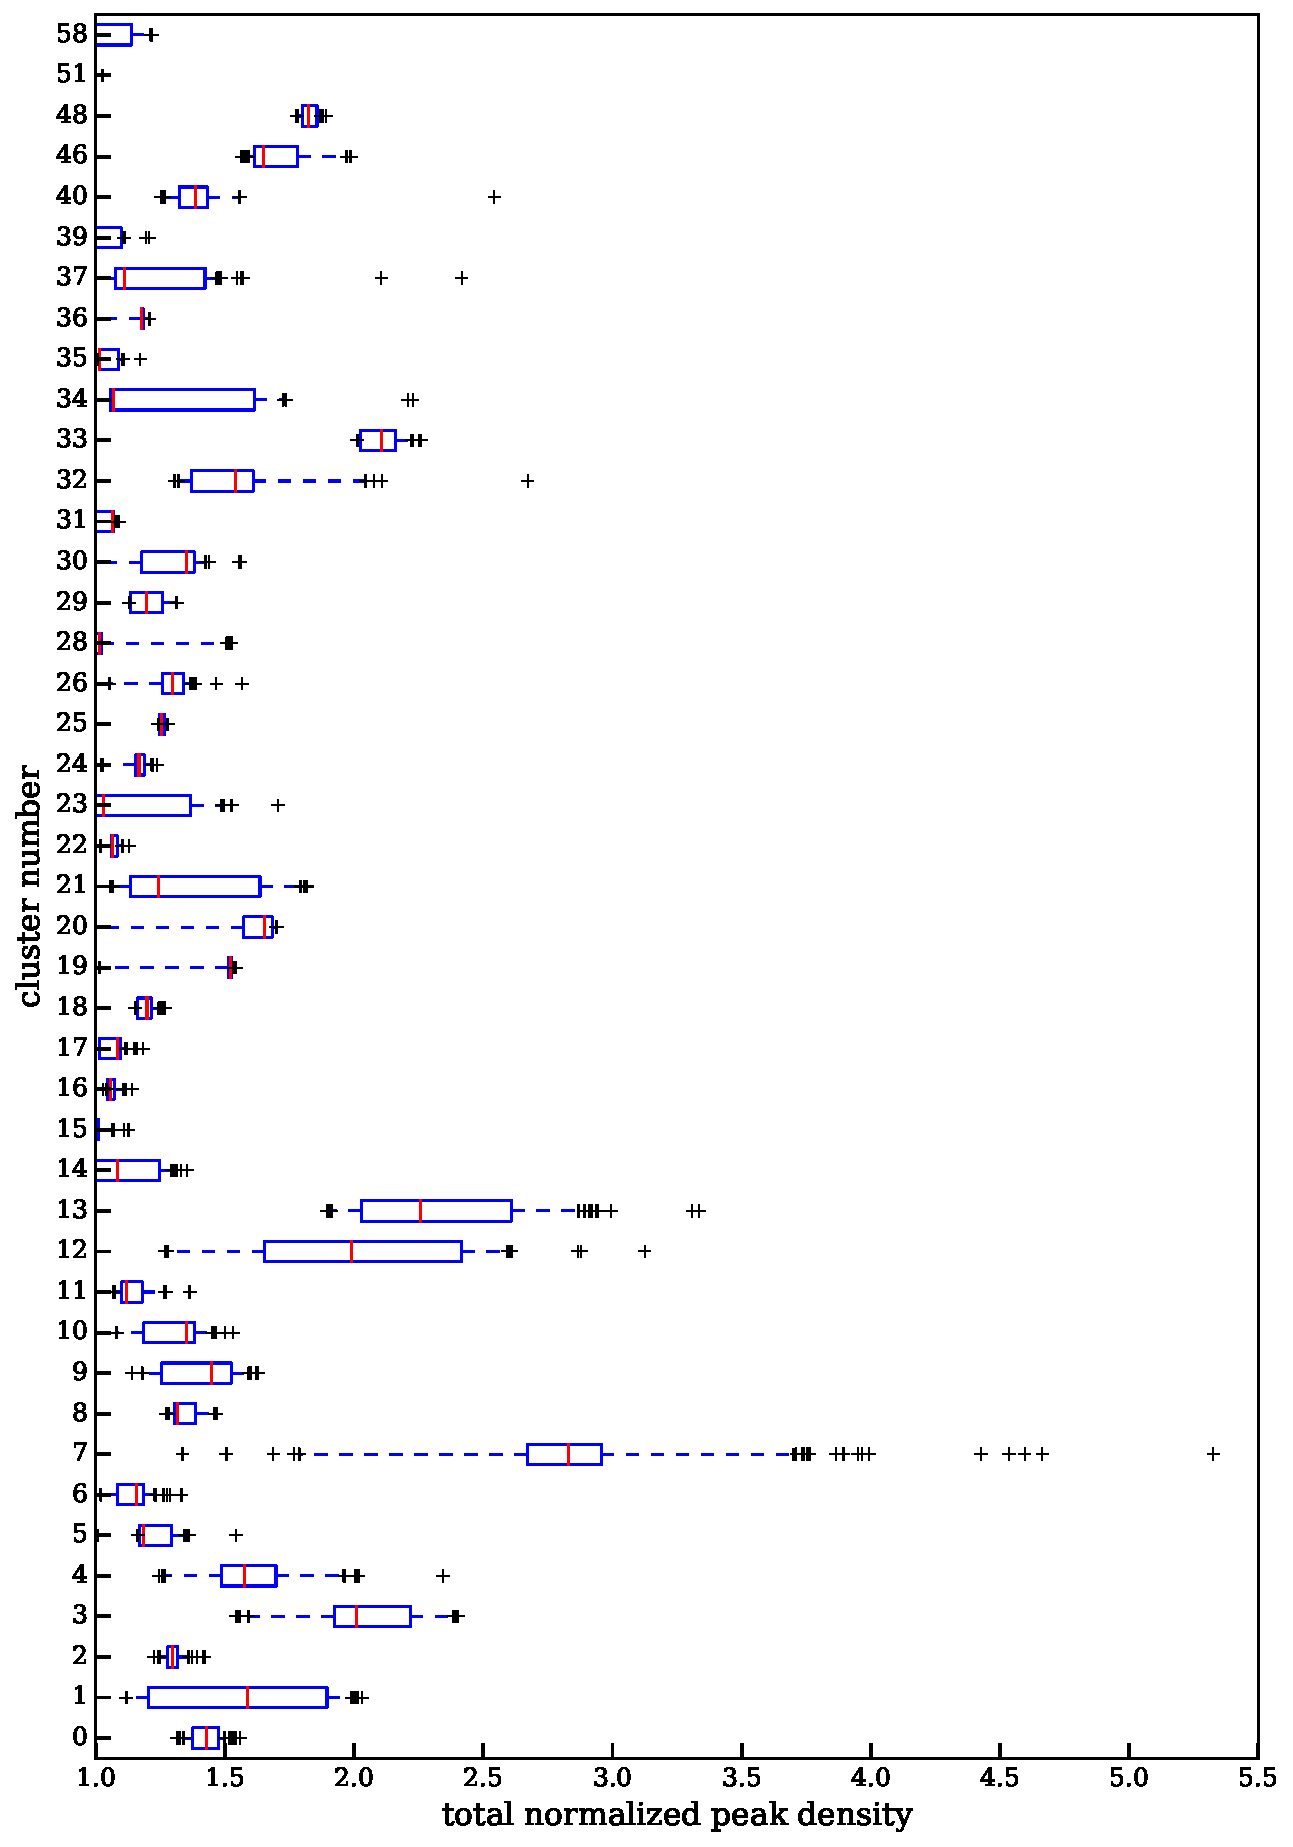
\includegraphics[width=0.85\linewidth]{fig8_total_normalized_peak_density.pdf}
	\caption{A box plot showing the distribution of the total normalized peak density 
		for each cluster 
		based on 768 projections. The red line shows the median of the projections,
		the box encompasses the 25\% and 75\% percentile of the distribution while
		the whiskers mark the 5\% and the 95\% percentile. The other black crosses
		are data points with extreme values beyond the 5\% and 95\% percentile.
		\label{fig:total_peak_dens_distribution}
	}
\end{center}
\end{figure*}

\begin{table*}
	\begin{center}
	\caption{Summary statistic characterizing the offset distributions
		between the most bound particle and various summary statistics of 
		the member galaxy population
	\label{tab:most_bound_particle_offset_distributions}}
	\begin{tabular}{lrrrrrrr}
\toprule
{} &  location &  lower 68\% &  lower 95\% &  lower 99\% &  upper 68\% &  upper 95\% &  upper 99\% \\
\midrule
$\Delta y_{\rm BCG}$       &         0 &           -2 &          -2 &        -252
&          2 &         528 &        1107 \\
$\Delta y_{\rm centroid}'$ &         0 &        -134 &        -491 &       -1176 &         134 &         491 &        1176 \\
$\Delta y_{\rm KDE}'$      &         0 &         -19 &         -82 &       -1182 &          19 &          82 &        1182 \\
$\Delta y_{\rm num.dens}$  &         0 &         -83 &        -302 &       -1114 &          83 &         302 &        1114 \\
$\Delta y_{\rm shrink}'$   &         0 &         -50 &        -288 &       -1025 &          50 &         288 &        1025 \\
\bottomrule
\end{tabular}

\end{center}
\small{The offsets represented with the prime $'$ symbols are estimated using the luminosity weighted galaxy 
data.}
\end{table*}


\begin{table}
	\begin{center}
	\caption{Summary statistic characterizing the offset distributions
		for between the DM peak and the estimated galaxy location. 
		All 43 clusters and all 768 projections are used in this table. 
		The highest density values were used for the computation when there were more
		than one peak value estimated from the KDE.
	\label{tab:offset_distributions}}
	\begin{tabular}{lrrrrrrr}
\toprule
kpc &  mean &  std &   min &  25\% &  50\% &  75\% &  max \\
\midrule
$|\Delta s_{\rm BCG}|$       &    69 &  294 &     0 &    2 &    3 &    7 & 2335 \\
$\Delta x_{\rm BCG}$         &   -14 &  226 & -2331 &   -2 &   -0 &    1 & 2327 \\
$\Delta y_{\rm BCG}$         &    23 &  197 & -1980 &   -2 &    0 &    2 & 2332 \\
$|\Delta s_{\rm centroid}'|$ &   261 &  209 &     2 &  114 &  202 &  317 & 1103 \\
$\Delta x_{\rm centroid}'$   &   -42 &  224 & -1022 & -164 &  -37 &   66 & 1101 \\
$\Delta y_{\rm centroid}'$   &     0 &  244 & -1102 & -111 &   -0 &  111 & 1100 \\
$|\Delta s_{\rm shrink}'|$   &   118 &  156 &     0 &   21 &   60 &  165 & 1454 \\
$\Delta x_{\rm shrink}'$     &    -7 &  131 & -1089 &  -39 &   -3 &   23 &  969 \\
$\Delta y_{\rm shrink}'$     &     0 &  145 & -1091 &  -32 &    0 &   32 & 1109 \\
$|\Delta s_{\rm KDE}'|$      &    37 &   35 &     0 &   14 &   26 &   49 &  498 \\
$\Delta x_{\rm KDE}'$        &    -2 &   35 &  -330 &  -17 &   -2 &   12 &  386 \\
$\Delta y_{\rm KDE}'$        &    -0 &   37 &  -439 &  -15 &    0 &   15 &  440 \\
$\Delta s_{\rm num. KDE}$    &   136 &  161 &     1 &   56 &   92 &  147 & 2126 \\
$\Delta x_{\rm num. KDE}$    &   -12 &  142 & -1967 &  -55 &   -4 &   53 &  993 \\
$\Delta y_{\rm num. KDE}$    &    -0 &  155 & -1415 &  -54 &   -0 &   54 & 1417 \\
\bottomrule
\end{tabular}

\end{center}
\small{The offsets represented with the prime $'$ symbols are estimated using the luminosity weighted galaxy 
data.}
\end{table}






\clearpage\bsp\label{lastpage} 
\end{document}
